\chapter{An Introduction to Linear QPL}\label{chap:informalintroductionLinearQuantumProgrammingLanguage}
\lstset{style=inlinqpl}
\section{Introduction to \lqpl}\label{sec:introlqpl}
This chapter  presents an overview of the linear quantum
programming language. Explanations of \lqpl{} programs, statements, 
and expressions are given.


\lqpl{} is  a language for experimenting with  quantum
algorithms. The language provides an expressive syntax for creating functions 
and defining and working
 with different datatypes. \lqpl{} has \qubit{}s as first class
citizens of the language, together with quantum control. 
Classical operations and classical control are also available to 
work with classical data.

The language design started from QPL in \cite{selinger04:qpl}
and rapidly evolved to a point where a direct comparison is 
somewhat difficult.
Major differences are the type system, the syntax and structure of functions
and the choices of individual statements.

\subsection{Functional versus imperative}\label{subsec:lqplfunctionvsimperative}
\lqpl{} is a functional language that uses single assignment. It resembles
QPL in this aspect rather than QML of \cite{alti05:functionalQMLlics}. 
Single assignment means that a variable always has a unique value until its
use. (See \ref{subsec:lqpllinearity} below.)

Like most functional languages, side effects are not allowed in functions, 
\emph{other than those that occur due to quantum entanglement}. Side effects in imperative languages
are those where a global variable is updated or values are read or written. 
An example of this in an imperative
 quantum language is a procedure in QCL from 
\cite{omer:2000}. \lqpl{} does not have the concept of a global variable. 
Currently, I/O is undefined.  Side effects from quantum entanglement can 
occur when a \qubit{} is passed as a parameter to a function and it is
operated on in the function.

\subsection{Linearity of \lqpl}\label{subsec:lqpllinearity}
The language \lqpl{} treats all quantum variables as \emph{linear}. This 
means that any variable \emph{may only be used once}. 
The primary reason for implementing this is the underlying aspect of 
linearity of quantum systems, as exemplified by 
 the \emph{no-duplication} rule which must be respected at all times. 
This allows us to provide
compile-time checking that enforces this rule.

The compiler and language do
 provide ways to ``ease the burden'' of linear thinking. 
For example, function calls (see \vref{subsec:functioncalls}) 
provide a specialized syntax for variables
which are both input and output to a function. The ability to use
a classical value (integer or boolean) multiple times is handled by  
\inlqpl{use} statements (see \vref{subsec:usestatements}), which place values on to the
classical stack where the values may be used multiple times.

\begin{figure}[htbp]
\lstinputlisting[style=linqpl]{examplecode/LengthList.qpl}
\caption{\lqpl{} code to return the length of the list}\label{fig:lenSQPL}
\end{figure}

An example illustrating linearity is given in \vref{fig:lenSQPL}. In
line \ref{line:lengthlist:len}, the function \inlqpl{len} is defined
as taking one argument of type \inlqpl{List(a)} and returning
a variable of type \inlqpl{Int}. The input only argument, \inlqpl{listIn},
\emph{must be destroyed in the function}. When the
case statement refers to \inlqpl{listIn}, the argument is 
destroyed, fulfilling the requirement of the function to do so.




\section{\lqpl{} programs}\label{sec:lqplprograms}
\lqpl{} programs  
consist of combinations of functions and data definitions, with 
one special function named \inlqpl{main}. 
The functions and data definitions are
\emph{simultaneously declared} and  so may be 
given in any order. The program will start executing at the \inlqpl{main}
 function. 

A physical program will typically consist of one or more source files
with the suffix \terminalio{.qpl}. Each source file may contain
functions and data definitions. It  may also
 \emph{import} the contents of other 
source files. The name of a source file is not significant in \lqpl. 
Common practice is to have one significant function per source file
and then to import all these files into the source file containing
the \inlqpl{main} function.

The above structure was chosen thinking of Haskell 
 \cite{peyton2003:haskell98} and C \cite{kernighan:c}. Global definitions 
of functions and types is borrowed from Haskell, while the \inlqpl{main} 
start point and import feature is a combination of Haskell and C.

\subsection{Data definitions}\label{subsec:datadefinitions}
\lqpl{} provides the facilities to define  datatypes with 
a syntax reminiscent of Haskell \cite{peyton2003:haskell98}. 

Natively, the language provides \inlqpl{Int}, 
\inlqpl{Qubit} and \inlqpl{Bool} 
types. \inlqpl{Bool} is the standard Boolean  type with values
\inlqpl{true} and \inlqpl{false}. \inlqpl{Int} is a standard 32-bit
integer. \inlqpl{Qubit} is a single \qubit{}.

In \lqpl{} both native types and other constructed datatypes may
be used in the definition of
constructed datatypes. These constructed datatypes may involve
 sums, products,
singleton types and parametrization of the constructed type.
For example, a type that is the sum of the integers and the Booleans
can be declared as  follows:
\begin{lstlisting}[style=linqplnonum]
        qdata Eitherib = {Left(Int) | Right(Bool)}
\end{lstlisting}
The above example illustrates the basic syntax of the 
data declaration. 
\paragraph{Syntax of datatype declarations.}
Each datatype declaration must begin with the keyword \inlqpl{qdata}. This is
followed by \emph{the type name}, which must be an identifier 
starting with an uppercase letter. The type name may also be followed by
 any number of \emph{type variables}. Type variables must be and identifier starting
with a lower case letter. Typically, a single letter is used.
This is then followed by an equals sign
and   completed by a list of \emph{constructors}. The list of constructors
must be surrounded by 
braces and each constructor must be separated from the others 
by a vertical bar. Each constructor is followed by an optional parenthesized
list of \emph{simple types}. 
Each simple type is either a built-in type, (one of 
\inlqpl{Int, Bool, Qubit}), a type variable that was used in the
type declaration, or another declared type, surrounded by 
parenthesis. \lqpl{} allows recursive
references to the type currently being declared. All constructors must
begin with an upper case letter. Constructors and types are in different
namespaces, so it is legal to have the same name for both. For example:
\begin{lstlisting}[style=linqplnonum]
       qdata Record a b = {Record(Int, a, b)}
\end{lstlisting}
In the above type definition,
 the first ``\inlqpl{Record}'' is the type, while the second is the 
constructor. The triplet ``\inlqpl{(Int,a,b)}'' is the product of the
type \inlqpl{Int} and the type variables \inlqpl{a} and \inlqpl{b}.
Since constructors may reference their own type and other 
declared types, recursive 
data types such as lists and various types of
 trees may be created:

\begin{lstlisting}[style=linqplnonum]
        qdata List a   = {Nil     | Cons(a, List(a))}
        qdata Tree a   = {Leaf(a) | Br(Tree(a), Tree(a))}
        qdata STree a  = {Tip     | Fork(STree(a), a, STree(a))}
        qdata Colour   = {Red     | Black}
        qdata RBSet a  = {Empty   |
	                  RBTip(Colour, RBSet(a), a, RBSet(a))}
        qdata RTree a  = {Rnode(a, List(a))}
        qdata Rose a   = {Rose(List(a, Rose(a)))} 
\end{lstlisting}
\subsection{Function definitions}\label{subsec:functiondefinitions}
Function definitions may appear in any order within a
\lqpl{} source file. 
\paragraph{Syntax of function definitions.} 
The first element of a function definition is
\emph{the name}, an identifier starting with a 
lower case letter. This is always followed by a double semi-colon and 
\emph{a signature}, which details the type and characteristics 
of input and output arguments. The final component of the 
function definition is
\emph{a body}, which is a block of \lqpl{} statements. 
Details of statements are given in \vref{sec:lqplstatements}.

The structure of function definitions is unique to \lqpl, although
broadly based on one of the acceptable syntaxes for C function definitions
as in \cite{kernighan:c}. The major difference occurs in the signature
which, as will be seen below, allows for both classical and quantum input
arguments and specifies the quantum outputs of a function. Another difference
is that \lqpl{} defines all functions globally, hence there is no
requirement for declarations separate from the definitions.

Let us examine two examples of functions. The first, in \vref{fig:defsec:gcd}
 is a fairly 
standard function to determine the greatest common divisor of two 
integers.

\begin{figure}[htbp]
\begin{singlespace}
\lstinputlisting[style=linqpl]{examplecode/gcd.qpl}
\end{singlespace}
\caption{\lqpl{} function to compute the GCD}\label{fig:defsec:gcd}
\end{figure}

The first line has  the name of the function, \inlqpl{gcd}, a separating double colon, and
 the signature. 
The signature of the function is  \inlqpl{(a:Int, b:Int | ; ans:Int)}.
This signature tells the compiler that \inlqpl{gcd} expects
two input arguments, each of type \inlqpl{Int} and that they are
 \emph{classical}. The compiler deduces this
from the fact that they both appear before the '\inlqpl{|}'.
In this case there are no  quantum input arguments
as there are no parameters between the '\inlqpl{|}' and the
'\inlqpl{;}'. The last parameter tells us that this function returns
one quantum item of type \inlqpl{Int}. Returned items are always  
quantum data.

The signature specifies variable names for the parameters
 used in the body. All input parameters are available as variable
names in expression and statements. Output parameters are available to be
assigned and, indeed, must be assigned by the end of the function.


The next example, in \vref{fig:defsec:inttoqubit}
 highlights the linearity of variables in \lqpl. This function is 
 used to create a list of \qubit{}s corresponding to the
\bit{} representation of an input integer.

At line 1,  the program uses the import command.
\inlqpl{#Import} must have a file name directly after it. This 
command directs the compiler to stop reading from the current file
and to read  code in the imported file until the end of that
file, after which it  continues with the current 
file.  The compiler will not reread the same file in a single
 compilation, and it will import from any file.


\begin{figure}[htbp]
\begin{singlespace}
\lstinputlisting[style=linqpl]{examplecode/intToQubitList.qpl}
\end{singlespace}
\caption{\lqpl{} function to create a \qubit{} register}
\label{fig:defsec:inttoqubit}
\end{figure}

For example, consider a case with three source files, A, B and C.
Suppose file A has import commands for both B and  C, with B being
imported first. Further suppose that  file B 
 imports C. The compiler will start reading A, suspend at the first 
import and start reading B. When it reaches B's \inlqpl{#Import} of C, it
will suspend the processing of B and read C. 
After completing the read of C, the compiler
reverts to processing B.
After completing the read of B, the compiler does a 
final reversion and finishes  processing  A. 
However, when A's \inlqpl{#Import} of C
is reached, the compiler will ignore this import
 as it keeps track of the fact C has
already been read.

In the signature on lines 
\ref{line:itqlfunctionstart}-\ref{line:itqlfunctionend},  
the function accepts
one quantum parameter of type \inlqpl{Int}. It returns
a  \inlqpl{Qubit} list and an \inlqpl{Int}. The integer returned, in
this program, is computed to have 
the same value as the one passed in. If this had not been
specified in this way, 
\emph{the integer would have been destroyed by the function}.  Generally, any usage
of a quantum variable destroys that variable. 

In the body of the function, note the \inlqpl{use n} in the
 block of statements. This allows  repeated 
use of the variable \inlqpl{n} at lines \ref{line:itqln0}, \ref{line:itqln1},
\ref{line:itqln2}, \ref{line:itqln3} and \ref{line:itqln4}. In these uses,
\inlqpl{n} is a classical variable, no longer on the quantum stack. The last
usage on line \ref{line:itqln4} where \inlqpl{n} is assigned to itself, 
returns \inlqpl{n} to the quantum world.




\section{\lqpl{} statements}\label{sec:lqplstatements}
The \lqpl{} language has  the following statements:
\begin{description}
\item{\emph{Assignment}:} The assign statement, e.g. \inlqpl{x = t};
\item{\emph{Classical control}:} The
\inlqpl{if} - \inlqpl{else} statement.
\item{\emph{Case}:} The \inlqpl{case} for operating on constructed
data types.
\item{\emph{Measure}:} The \inlqpl{measure} statement which measures
a \qubit{} and executes dependent statements.
\item{\emph{Use}:} The
\inlqpl{use} and classical assign statements which operate on classical
data, moving it on to the classical stack for processing.
\item{\emph{Function calls}:} The various ways of calling functions or applying
transformations.
\item{\emph{Blocks}:} A group
of statements enclosed by '\{' and '\}'.
\item{\emph{Quantum control}:} Control of statements by 
 the \inlqpl{<=} qualifier.
\item{\emph{Divergence}:} The \inlqpl{zero} statement.
\item{\emph{Other}:} the \inlqpl{discard} statement.
\end{description}

Most of these correspond to the conceptual statements for quantum 
pseudo-code as given in \cite{knill96:conventions}.

\subsection{Assignment statement}\label{subsec:assignmentstatement}
Assignments create variables. Typical
examples of these are:
\begin{lstlisting}
        q1  = |0>;
        i   = 42;
        bt1 = Br(Leaf(q1), Br(Leaf(|0>), Leaf(|1>)));
\end{lstlisting}
Here the first line creates a \qubit{}, \inlqpl{q1}, 
with initial value \ket{0}. The
second line creates an integer ,\inlqpl{i},
  with the value $42$. The last line creates a
binary tree, \inlqpl{bt1},
 with \inlqpl{q1} as its leftmost node, and the right node
being a sub-tree with values \ket{0} and \ket{1} in the left and 
right nodes respectively. Note that after the execution of the 
third statement, the variable \inlqpl{q1} is no longer in scope so the
name may be reused by  reassigning some other value to it.

The variables  on the left hand side of an
assignment are always quantum variables.
\paragraph{Syntax of assignment statements.} An assignment statement always
begins with an \emph{identifier}. This
must be followed by a single equals sign and then an \emph{expression}.
Expressions are introduced and defined  in \vref{sec:lqplexpressions}

Identifiers in \lqpl{} must always start with a lower case letter.


\subsection{Classical control}\label{subsec:classicalcontrolstatements}
Classical control provides a way to choose sets of instructions
to execute based upon the values on the classical stack. 

\begin{figure*}[htbp]
\begin{singlespace}
\lstinputlisting[style=linqpl]{examplecode/lowprime.qpl}
\end{singlespace}
\caption{\lqpl{} program demonstrating \inlqpl{if-else}}
\label{fig:defsec:stmts:demoofifelse}
\end{figure*}

The expressions in the selectors 
\emph{must} be classical. This means they can only consist of
operations on  constants and classical identifiers. 
It is a semantic error to 
have an expression that depends on a
quantum variable. For an example, see the code to determine if
an input number is a small prime in \vref{fig:defsec:stmts:demoofifelse}.

Some form of classical control is encountered in all current quantum 
programming languages. It is central to the semantics of \cite{selinger04:qpl}.
Note that many languages also include a classically controlled 
looping statement (such as \inlqpl{while} or \inlqpl{do}). \lqpl{} 
does not, relying on recursive functions to achieve the same end.

\paragraph{Syntax of the \inlqpl{if -} \inlqpl{else} statement.} 
The statement starts
with the word \emph{if}, followed by one or more \emph{selectors}.
Each selector is composed of a classical Boolean expression $e_b$, the
symbols \emph{=>} and a dependent block. 
 The statement is 
completed by a special selector where the Boolean expression is
replaced with the word \emph{else}. 

In the list of $e_i => b_i$ selectors, 
$b_i$ is executed only when $e_i$ is the first expression to
evaluate to \inlqpl{true}. All others are skipped. The final 
grouping of \inlqpl{else =>} \emph{block} is a default and will be
executed when all the  selector expressions in a list
  evaluate to \inlqpl{false}.

When writing the dependent blocks of the selectors,
 quantum variable creation must be
the same in each block.
 The compiler will give you a semantic
warning if a quantum variable is created in one branch and not another.


\subsection{Measure statement}\label{subsec:measurestatements}

The \inlqpl{measure} statement performs a measurement of a \qubit{} and
executes code depending on the outcome. Currently in \lqpl{}, all
measures are done with respect to the basis $\{\ket{0},\ket{1}\}$. 
Referring to  \vref{fig:defsec:coin}, there is a
\inlqpl{measure} on line \ref{line:cflipmeasure}. 


%\begin{wrapfigure}{l}{3in}
\begin{figure}[htbp]
\centering
\subfloat[Coin flip code]{
\begin{singlespace}
\lstinputlisting[style=linqpl]{examplecode/coin.qpl}
\end{singlespace}}\qquad
\subfloat[Stack machine state at end]{
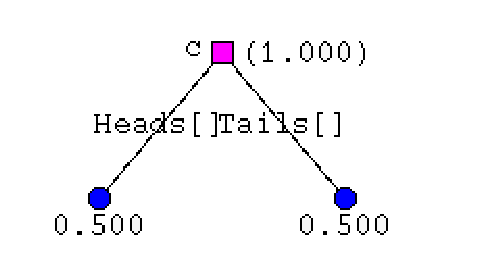
\includegraphics[scale=.6]{images/headOrTails.eps}
}
\caption{\lqpl{} program to do a coin flip}\label{fig:defsec:coin}
\end{figure}

Consider the  program in \ref{fig:defsec:coin} which emulates a coin flip.
In the function \inlqpl{cflip},  a \qubit{} is prepared by initializing it
to \ket{0} and applying the \Had{} transform. This creates a \qubit{} 
whose density matrix is {\begin{singlespace}$\begin{pmatrix}.5&.5\\ 
.5&.5\end{pmatrix}$\end{singlespace}}. When
 this \qubit{} is measured, it has a $50\%$ chance of being $0$ and 
an equal chance of being $1$. 

In the branches of the measure,  different values are assigned to the 
return variable $c$. Each of these assignments happens with a probability of
$50\%$. Once the measure statement is completed, the variable \inlqpl{c}
will be \inlqpl{Heads} and \inlqpl{Tails} each with a probability of $50\%$.
In the quantum stack machine this is represented as in 
sub-figure b of \vref{fig:defsec:coin}.


This illustrates the largest difference between quantum and classical 
processing of choices. In classical programming languages, a choice such
as a case type statement 
\emph{will only execute the code on one of the branches of the case}. 
In \lqpl{}, \emph{every} branch may be executed.


%\begin{wrapfigure}{l}{3in}
\begin{figure}[htbp]
\centering
\subfloat[Balanced creation]{
\begin{singlespace}
\lstinputlisting[style=linqpl]{examplecode/dataCreationExample1.qpl}
\end{singlespace}}
\qquad
\subfloat[Unbalanced creation]{
\begin{singlespace}
\lstinputlisting[style=linqpl]{examplecode/dataCreationUnbalanced.qpl}
\end{singlespace}}
\caption{\lqpl{} programs contrasting creation}
\label{fig:defsec:balancedcreation}
\end{figure}

When writing the dependent blocks of \inlqpl{measure}
 (and \inlqpl{case} in \vref{subsec:casestatements}) 
 variable creation must be
the same in each dependent list of statements.
 The compiler will give you a semantic
warning if a variable is created in one branch and not another.

For example, consider \vref{fig:defsec:balancedcreation}. In the left 
hand program on the 
\inlqpl{measure} starting at line \ref{line:measure1}, each branch creates a 
variable named '\inlqpl{i}'. This is legal and from line \ref{line:iexists}
forward,  '\inlqpl{i}' will be available.

On the other hand, the measure in the right hand program  starting in line 
\ref{line:measure2} assigns to the variable  '\inlqpl{c}' in
the \ket{0} branch and  '\inlqpl{d}' in the \ket{1} branch. At line
\ref{line:neitherdorc}, neither variable will be available. The compiler
will give the warnings:
\begin{quote}
\footnotesize
\terminalio{Warning: Unbalanced creation, discarding c of type INT}\\
\terminalio{Warning: Unbalanced creation, discarding d of type INT}
\end{quote}

\paragraph{Syntax of the \inlqpl{measure} statement.} This statement
starts with the word \emph{measure}, 
followed by a variable name, which must be of type \inlqpl{Qubit}. 
Next, the keyword \emph{of} signals the start of the two case selections.
 The case selection starts with either \ket{0} or \ket{1}, followed by
\inlqpl{=>} and the block of dependent statements.

Note that \emph{both} case selections for a \qubit{} must be present. However,
it is permissible to not have any statements in a block.

\subsection{Case statement}\label{subsec:casestatements}
The \inlqpl{case} statement is used with any variable of a declared
datatype. 
\begin{figure}[htbp]
\begin{singlespace}
\lstinputlisting[style=linqpl]{examplecode/reverse.qpl}
\end{singlespace}
\caption[Reverse program to demonstrate \inlqpl{case}]{\lqpl{} program demonstrating \inlqpl{case}, a function to reverse a list.}
\label{fig:defsec:reverse}
\end{figure}  


In \vref{fig:defsec:reverse}, the program declares the
 \inlqpl{List} data type, which is parametrized by one
type variable and has two constructors: \inlqpl{Nil} which has no
arguments and \inlqpl{Cons} which takes two arguments of types
\inlqpl{a} and \inlqpl{List(a)} respectively.

The function \inlqpl{reverse} takes a list 
as an input argument and returns a single list, which is the original 
list in reverse order. Because of the linearity of the language
the original input list is not in scope at the end of the function.
The function \inlqpl{reverse} delegates to the function \inlqpl{rev'}
which uses an accumulator to hold the list as it is reversed.

The case statement begins on line \ref{line:rev:caserev}. For
\inlqpl{Nil}, it assigns the accumulator to the return list. For
\inlqpl{Cons}, it first adds the current element to the
front of the accumulator list, then it uses a recursive call
to reverse the tail of the original list with the new accumulator.


\begin{figure}[htbp]
\begin{singlespace}
\lstinputlisting[style=linqpl]{examplecode/treeMaxDepth.qpl}
\end{singlespace}
\caption[Tree depth program to demonstrate \inlqpl{case}]{\lqpl{} program demonstrating \inlqpl{case}, a function to compute the max tree depth.}
\label{fig:defsec:treemaxdepth}
\end{figure}

Consider the example in \vref{fig:defsec:treemaxdepth}. \inlqpl{TTree}
is a parametrized data type which depends on 
the type variable \inlqpl{a}. It
 has three constructors: \inlqpl{Tip} which takes no arguments;
\inlqpl{Br} which takes three arguments of types \inlqpl{TTree a, a} and
\inlqpl{TTree a}; and \inlqpl{Node} which takes one argument of type
\inlqpl{a}.

In \inlqpl{treeMaxDepth}, the case statement on line
\ref{line:flattenTree:casedepth} illustrates a ``don't care'' pattern for
both the \inlqpl{Node} and \inlqpl{Br} constructors. This function
 returns the maximum depth of the \inlqpl{TTree} and actually
discards  the actual data elements stored at nodes.



\paragraph{Syntax of the \inlqpl{case} statement.} This statement
starts with the word \emph{case}, 
followed by a variable   of some declared type.
Next, the keyword \emph{of} signals the start of the case selections.
The number of constructors in a type determine how many 
case selections the statement has. There is one selection 
for each constructor.
Each case selection consists of  a \emph{constructor pattern}, a
'\inlqpl{=>}' and dependent statements. 

Constructor patterns 
are the constructor followed by a parenthesized list of 
variables and / or \emph{don't care} symbols, '\_'.  Non-parametrized 
constructors appear without a list of variable names. The 
don't care symbol causes data to be discarded.

\subsection{Use and classical assignment statements}\label{subsec:usestatements}

The \inlqpl{use} statement is used with any variable of type \inlqpl{Int}
or \inlqpl{Bool}. 
This statement  has a single 
set of dependent statements. These may 
either be explicitly attached to the \inlqpl{use} statement or implicit.
Implicit dependent statements are all the statements following
the \inlqpl{use} until the end of the current block. 

Classical assignment is grouped here as it is syntactic sugar for a
\inlqpl{use} with implicit statements. This is illustrated in 
\ref{fig:useequalsassignment}.

%\begin{wrapfigure}{l}{2.75in}
\begin{figure}[htbp]
\begin{singlespace}
\begin{center}
\begin{tabular}{lcl}
$\vdots$ & & $\vdots$ \\
\begin{lstlisting}
i := exp;
s1;
\end{lstlisting} &
$\equiv$ &
\begin{lstlisting}
i = exp;
use i;
s1;
\end{lstlisting} \\
$\vdots$ & & $\vdots$
\end{tabular}
\end{center}
\end{singlespace}
\caption{Syntactic sugar for \inlqpl{use} / classical assignment}
\label{fig:useequalsassignment}
\end{figure}

The three types of classical use are semantically equivalent, but
do have different syntaxes as illustrated in \vref{fig:defsec:usestatements}.

\begin{figure}[htbp]
\centering
\subfloat[Explicit dependence]{
\begin{singlespace}
\lstinputlisting[style=linqpl]{examplecode/treeMaxDepth.explicit.frag.qpl}
\end{singlespace}}
\qquad
\subfloat[Implicit dependence]{
\begin{singlespace}
\lstinputlisting[style=linqpl]{examplecode/treeMaxDepth.frag.qpl}
\end{singlespace}}
\qquad
\subfloat[Classical assign]{
\begin{singlespace}
\lstinputlisting[style=linqpl]{examplecode/treeMaxDepth.cassign.frag.qpl}
\end{singlespace}}
\caption{Fragments of \lqpl{} programs contrasting \inlqpl{use} syntax}
\label{fig:defsec:usestatements}
\end{figure}

In sub-figure (a) of \ref{fig:defsec:usestatements}, the \inlqpl{use}
statement starts on line \ref{line:tmdfragexplicit:use}. The next two
statements are explicitly in its scope, which ends at line 
\ref{line:tmdfragexplicit:scopend}.  In sub-figure (b) of the same figure,
the \inlqpl{use} at line \ref{line:tmdfrag:use} is implicit. Its scope
extends to line \ref{line:tmdfrag:scopend}. Finally, in sub-figure(c),
the same effect is achieved with two classical assignments at 
lines \ref{line:tmdfragcas:assignj} and \ref{line:tmdfragcas:assignk}.
The scope of these assignments extend to line \ref{line:tmdfragcas:scopend}.


Unlike data types and \inlqpl{Qubit}s, which have a maximum number of 
sub-stacks, an \inlqpl{Int} has the potential to have 
 an unbounded number of values and therefore sub-stacks. 
The dependent statements of
 the \inlqpl{use} statement are executed for \emph{each} 
of these values.

To execute different statements depending on the value of 
the \inlqpl{Int}, \lqpl{}
provides the \inlqpl{if} - \inlqpl{else} statement as discussed in
\vref{subsec:classicalcontrolstatements}. Typical use would be immediately
after the \inlqpl{use} statement, or as the first statement of
the dependent block of an explicit \inlqpl{use} statement.

\paragraph{Syntax of the \inlqpl{use} statement.} This statement starts with 
the word \inlqpl{use},
 followed by a list of variable names, which must be  of
type \inlqpl{Int} or \inlqpl{Bool}. If there is an 
explicit dependent block for the statement, it is given by the
keyword \inlqpl{in} followed by the dependent block.

When the \inlqpl{use} statement is \emph{not} followed by a dependent block, 
the rest of the statements in the enclosing block are considered in
the scope of the \inlqpl{use}.

Classical assign syntax is a variable name, followed by the 
symbol '\inlqpl{:=}' followed by an expression. The expression must have
type \inlqpl{Int} or \inlqpl{Bool}. 

\subsection{Function calls}\label{subsec:functioncalls}
Function calls include calling functions defined in  programs and
the predefined transforms. The list of predefined transforms valid
in a \lqpl{} program are given in \vref{tab:lqpltransforms}.
%TODO - Dr. C regarding transforms
% - reduce primitives, show how to get rest
% - Explain interdependence
% - reexamine formula for Rot, possibly use R(n,t) (t  an int), = 1 &0\\0&e^{-i t \pi / 2^{n-1}}
% - Remove RhoZ, Phase, T (Rot...) and Swap (=, =)
\begin{table}
\centerline{
\begin{tabular}{|l|l|c|}
\hline
\textbf{\lqpl{}}& \textbf{A.K.A.} & \textbf{Matrix} \\
\hline 
& & \\
\inlqpl{Not} & $X$, Pauli-X, $\rho_X$  & $ 
\begin{bmatrix}
0&1\\
1&0
\end{bmatrix}$ \\ & & \\\hline
 & &  \\
\inlqpl{RhoY} & $Y$, Pauli-Y, $\rho_Y$ &
$ 
\begin{bmatrix}
0&-i\\
i&0
\end{bmatrix}$ \\ & & \\\hline
 & &  \\
\inlqpl{RhoZ (=Rot(0))} & $Z$, Pauli-Z, $\rho_Z$ &
$ 
\begin{bmatrix}
1&0\\
0&-1
\end{bmatrix}$ \\ & & \\\hline
 & &  \\
\inlqpl{Had} & Had, $H$ &
$ 
\frac{1}{\sqrt{2}}\begin{bmatrix}
1&1\\
1&-1
\end{bmatrix}$ \\ & & \\\hline
& & \\
\inlqpl{Swap} & Swap &
$ 
\begin{bmatrix}
1&0&0&0\\
0&0&1&0\\
0&1&0&0\\
0&0&0&1
\end{bmatrix}$ \\ & & \\\hline
& & \\
\inlqpl{Phase (=Rot(2))} & $S$, Phase $\sqrt{Z}$ &
$
\begin{bmatrix}
1&0\\
0&i
\end{bmatrix}$ \\ & & \\\hline
& & \\
\inlqpl{T(=Rot(3))} & $T$, $\frac{\pi}{8}$, $\sqrt{S}$ &
$
\begin{bmatrix}
1&0\\
0&e^{i\pi/4}
\end{bmatrix}$ \\ & & \\\hline
& & \\
\inlqpl{Rot(n)} & $R_n$, Rotation &
$
\begin{bmatrix}
1&0\\
0&e^{2i\pi/2^n}
\end{bmatrix}$ \\ & & \\\hline
\end{tabular}
} 
\caption{\lqpl{} transforms}\label{tab:lqpltransforms}
\end{table}

In addition to the predefined transforms, \lqpl{}
 allows you to prefix any of the 
predefined transformations with the 
string \inlqpl{Inv-} to get the inverse transformation. Controlled versions 
of transforms are accomplished by the built-in control mechanism using \verb|<=|.

The signatures of transforms are dependent upon the size of the 
associated matrix. A $2\times 2$ matrix gives rise to the signature
\inlqpl{(q:Qubit ; q:Qubit)}. In general, a $2^n \times 2^n$ matrix
will require $n$ \qubit{}s in and out. The parametrized transforms such
as \inlqpl{Rot} will  require one or more integers as input.

\subsubsection{Syntax of function calls}\label{subsubsec:syntaxfunction}
There are three different calling syntaxes for functions:
\begin{enumerate}
\item{} \emph{Functional} --- $(y_1,\dots,y_m) = f(n_1,\dots,n_k\, |\, x_1,\dots,x_j).$
\item{} \emph{Procedural} ---  $f(n_1,\dots,n_k\, |\, x_1,\dots,x_j\, ;\, y_1,\dots,y_m).$
\item{} \emph{Transformational} --- $f(n_1,\dots,n_k )\ z_1\ z_2\ \dots\ z_j.$
\end{enumerate}


\paragraph{Functions with classical and quantum inputs.}
These functions  may be called\footnote{A function
call where a  single unparenthesized variable appears on the
left hand side of the equals
 is
 actually an assignment statement. The  right hand side of the assignment 
is a function expression.
See \ref{subsec:assignmentstatement} and \ref{subsec:expressioncalls} for further details.} in each of the
three ways.
\begin{lstlisting}[style=linqpl]
      f ::(c1:Int,c2:Int | q1:Qubit, i1:Int ; a:Qubit, b:Int) = {...}
      ...
         (a,b) = f(c1,c2 | q1,i2);
         f(c1,c2 | q1,i2; a,b);
         f(c1,c2) q i;
\end{lstlisting}

When a function is called in the transformational syntax, as on the last 
line of the above code, the arguments separated by spaces (\inlqpl{q i} in the example) are 
both passed into
the function as arguments and used as return variables. 
The arguments in the parenthesis ( \inlqpl{c1,c2} in our example),
\emph{must} be classical and a
 semantic error will result if a quantum variable is used.
If the number of in and out quantum arguments are not the same
or their types
do not match, this syntax is not available.


\paragraph{Functions which have no quantum input arguments.}
Functions which have only classical  inputs 
may be called in either the functional or procedural 
syntax. As there are no input quantum arguments, transformational
syntax is not allowed.

\begin{lstlisting}[style=linqpl]
      g :: (c1:Int, c2:Int | ; r:Int, d:Int) = {...}
      ...
        (a,b) = g(c1,c2 |);
        g(c1,c2 | ; a,b);
\end{lstlisting}


\paragraph{Functions which have no classical input arguments.}
Functions having only quantum  inputs may use
all three syntaxes. In this case, where the classical
variable list of arguments is empty, the ``|'' may 
be eliminated in procedural or functional calling, and the 
parenthesis may be eliminated in transformational calling.

\begin{lstlisting}[style=linqpl]
      h :: (q1:Int, q2:Int ; r:Int, d:Int) = {...}
      ...
        (a,b) = h(|c,d);
        (a,b) = h(c,d);
        h( | a,b ; c,d);
        h(a,b; c,d);
        h a b;
\end{lstlisting}



\paragraph{Linearity of function call arguments.}
Each input argument is no longer in scope after the function call. If 
the input is a simple identifier, the same identifier may be used in
the output list of the function. The transformational
syntax uses this technique to leave the variable names unchanged.

\paragraph{Syntactic forms of function and transform calls.}
In all three of the forms for function calling, the number and type
of input arguments must agree with the definition of the function.
Output identifiers must agree in number and their type is set according
to the definition of the functions output parameters. Output
variables are always quantum.

The  \emph{functional} syntax for function calling has three parts.
The first part is a parenthesized  list of variable names separated by 
commas.
The parenthesized list is then followed by an equals sign. The right hand side
 consists of the function name
followed by the  parenthesized  input arguments. The input arguments 
consists of two lists of arguments separated by '\inlqpl{|}'. The first
list consists of the classical arguments, the second of the quantum arguments.
Each argument must be a valid expression as defined 
in  \vref{sec:lqplexpressions}.
 If there are no classical arguments, the '\inlqpl{|}' is optional.


The  \emph{procedural} syntax for function calling starts with the
function name, followed by a parenthesized grouping of input and
output arguments.  As in the functional form, the list of classical input 
arguments are separated from the quantum ones by '\inlqpl{|}', which may
be eliminated when there are no classical arguments. The input arguments
are separated from the output arguments by '\inlqpl{;}'. 

The \emph{transformational} syntax starts with the
function name followed  by a parenthesized list of classical
expressions and then by a series of identifiers, separated by white space.
A requirement for using this syntax is that the
number and types of the input and output quantum arguments must be the same. 
The identifiers will be passed as input to the function and will be
returned by the function. The parenthesis for the list of classical
expressions may be eliminated when there are no classical parameters.


Function calls may also be expressions, which is discussed in
\ref{subsec:expressioncalls}.

\subsection{Blocks}\label{subsec:blocks}
Blocks are created by surrounding a list of statements with braces. A 
block may appear wherever a statement does.  All of the ``grouping''
types of statements require blocks rather than statements as their group.
See, for example, the discussion on \inlqpl{case} statements
in \ref{subsec:casestatements}.

\subsection{Quantum control}\label{subsec:quantumcontrol}

Quantum control provides a general way to create and use controlled unitary 
transforms in an \lqpl{} program. 
An example of quantum 
control is shown in the prepare and teleport functions in
 \vref{fig:defsec:stmts:demoofcontrol}.


\begin{figure*}[htbp]
\begin{singlespace}
\lstinputlisting[style=linqpl]{examplecode/teleport.qpl}
\end{singlespace}
\caption{\lqpl{} program demonstrating quantum control}
\label{fig:defsec:stmts:demoofcontrol}
\end{figure*}

\paragraph{Syntax of quantum control}
In \lqpl{} any statement, including block statements and 
procedure calls may be quantum controlled.
Semantically, this will  affect all transforms that occur within
the controlled statement, including
any of the transforms in a called function.
The  syntax is \emph{statement} 
followed by the symbols \emph{<=}, followed
by a list of identifiers.  These identifiers may 
be of any type, but are typically
either \qubit{}s or constructed data types with \qubit{} elements, such as a 
\inlqpl{List(Qubit)}. Additionally, any identifier may be preceeded by a 
tilde (\raisebox{-.8ex}{$\,\tilde{}\,$}) to indicate $0-$control. The default is 
$1-$control.

The identifiers that are controlling a statement can not be used
in the statement. Controlling identifiers are exempt from
linearity constraints in that they remain in scope after the
quantum control construction.

The effect of the control statement is that all \qubit{}s in the 
control list, or contained in items
in that list are used to control all unitary 
transformations done in the controlled
statement.

\subsection{Divergence}\label{subsec:nontermination}
To force the execution  of a program  to diverge, you can use the
\inlqpl{zero} statement. This will set the probability of the values of
a program to 0, and is interpreted as non-termination.

\subsection{Discard}\label{subsec:discard}
In some algorithms, such as  in recursive functions when they process
the initial cases of constructed data,
the algorithm does not specify any action. In these cases, the programmer
may need to examine the requirements of linearity with respect to 
any passed in parameters. Often, these will need to be explicitly
discarded in base cases of such algorithms.
This is done via the discard statement.
An example may be seen in \vref{fig:inverserotate}.

\section{\lqpl{} expressions}\label{sec:lqplexpressions}

Expressions in \lqpl{} are used in many of the statements discussed in
\vref{sec:lqplstatements}. The four basic types of expressions are
identifiers, constants, constructor expressions, and calling expressions.
Arithmetic and logical combinations of classical
constants and classical identifiers
are allowed. As well, constructor and calling expressions often  take
lists of other expressions as arguments.

\subsection{Constant expressions}\label{subsec:constantexpressions}
The possible constant expressions in \lqpl{} are shown in
\vref{tab:constantexpressions}. The category column in this table
contains the word ``Classical'' when the constant may be used in arithmetic
or Boolean expressions.

\begin{table}[htbp]
\begin{center}
\begin{singlespace}
\begin{tabular}{|l|l|l|}
\hline
\textbf{Expression} & \textbf{Type} & \textbf{Category} \\
\hline
\hline
\emph{integer} & \inlqpl{Int} & Classical \\
& & \\
\inlqpl{true} & \inlqpl{Bool} & Classical \\
& & \\
\inlqpl{false} & \inlqpl{Bool} & Classical \\
& & \\
\ket{0} & \inlqpl{Qubit} & Quantum \\
& & \\
\ket{1} & \inlqpl{Qubit} & Quantum \\
\hline
\end{tabular}
\end{singlespace}
\end{center}
\caption{Allowed constant expressions in \lqpl}
\label{tab:constantexpressions}
\end{table}

\subsection{Identifier expressions}\label{subsec:identifierexpressions}
These expressions are just the identifier name. While an
identifier may be used wherever an expression is expected, the reverse is not
true. As an example, in function calls, any of the input arguments may be
expressions but the output arguments \emph{must} be identifiers.

Identifier expressions may be either quantum or classical in nature.
As discussed in \vref{subsec:assignmentstatement}, an identifier is
first created by an assignment statement. When initially created, the
identifier is always quantum. Using it where a classical expression is
required will result in an error. When it is desired to operate on an
identifier classically, it must first be the object
of a  \inlqpl{use} statement.
In all statements in the scope of that \inlqpl{use} statement
the identifier will be considered classical. See \vref{subsec:usestatements}
for further information and examples.

\subsection{Constructor expressions}\label{subsec:constructorexpressions}
These expressions are used to create new instances of declared data types.
Consider this sample fragment of code.

{\begin{singlespace}
\begin{lstlisting}[style=linqpl]
        qdata TTree a = {Tip | Br(TTree(a), a, TTree(a)) | Node(a)}
        qdata List a  = {Nil | Cons(a, List(a))}

        qbtree  = Br(Tip, |1>, Br(Node(|0>), |1>, Node(|1>)));
        intlist = reverse(Cons(5,Cons(4,Cons(3,Cons(2,Cons(1,Nil))))));
\end{lstlisting}
\end{singlespace}
}

These statements create a tree as in \ref{fig:treeExample} and
the list $[1,2,3,4,5]$. Compare the logical representation of
\inlqpl{qbtree} as in \ref{fig:treeExample} versus how it is stored
in the quantum stack machine, shown in \vref{fig:treeExampleInQS}.
\begin{figure}[htbp]
\begin{center}
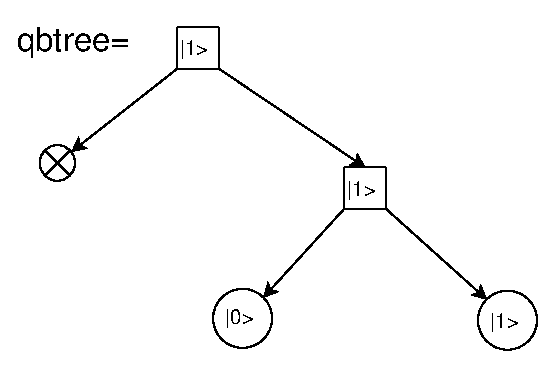
\includegraphics[scale=.6]{images/treeExample.eps}
\end{center}
\caption{Pictorial representation of \inlqpl{qbtree}}\label{fig:treeExample}
\end{figure}
\begin{figure}[htbp]
\begin{center}
\subfloat[After Running]{
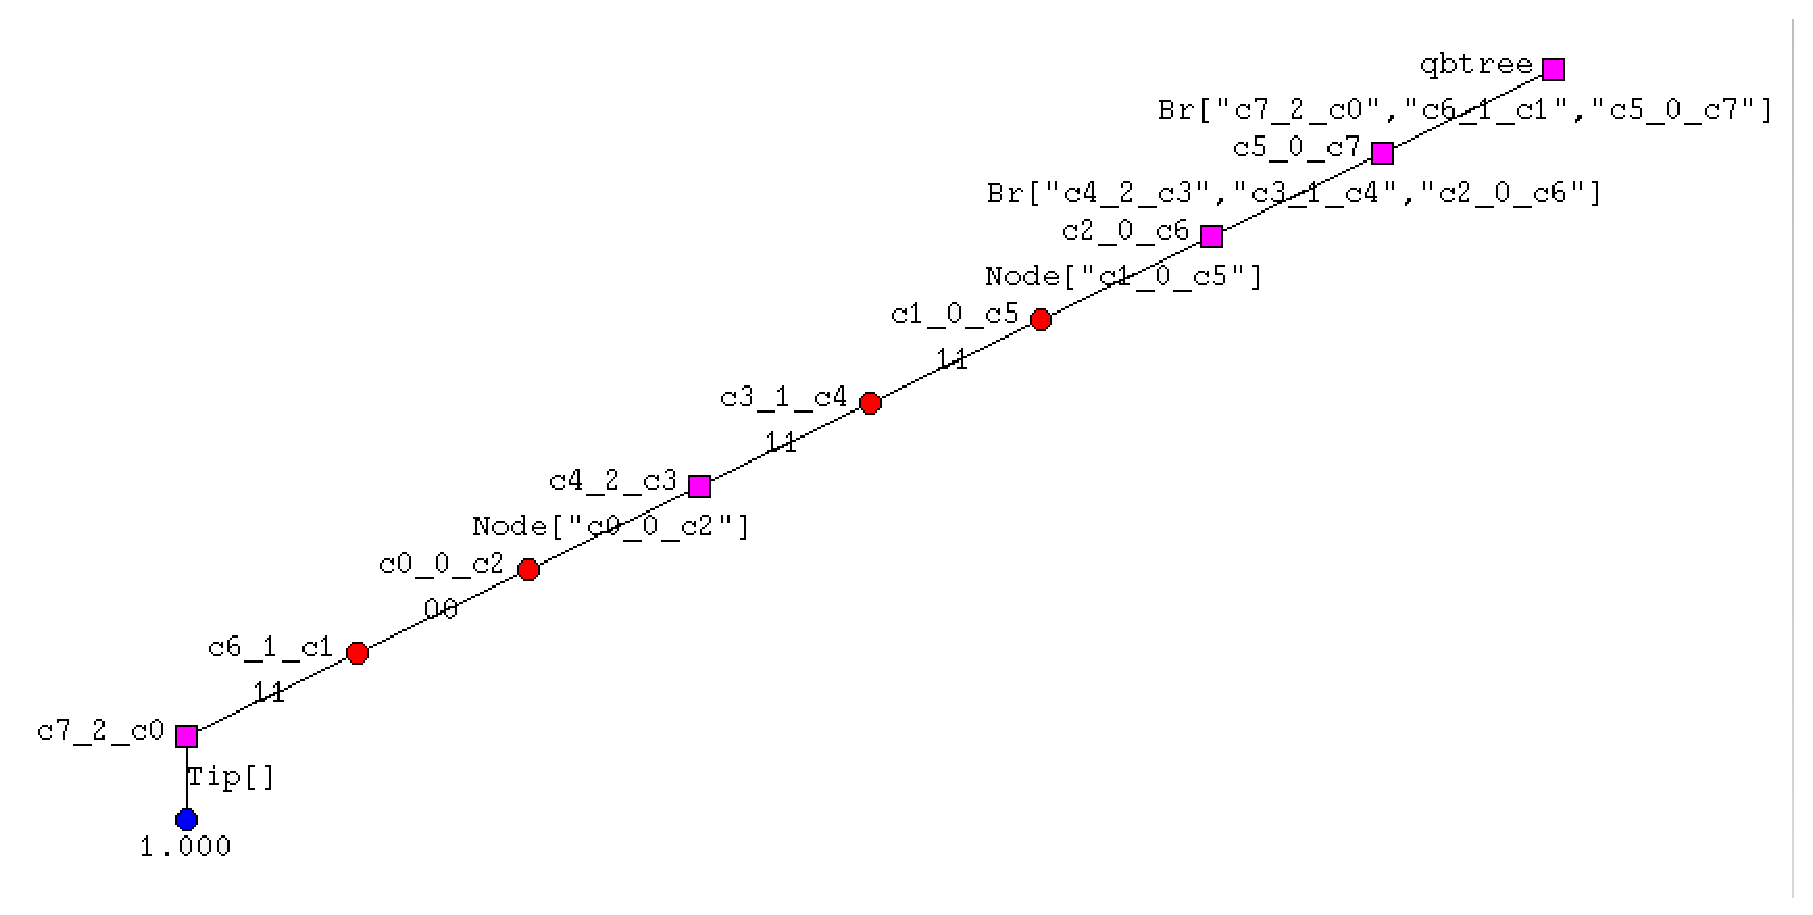
\includegraphics[scale=.5]{images/treeExampleInQS.eps}}
\qquad
\subfloat[Trimmed]{
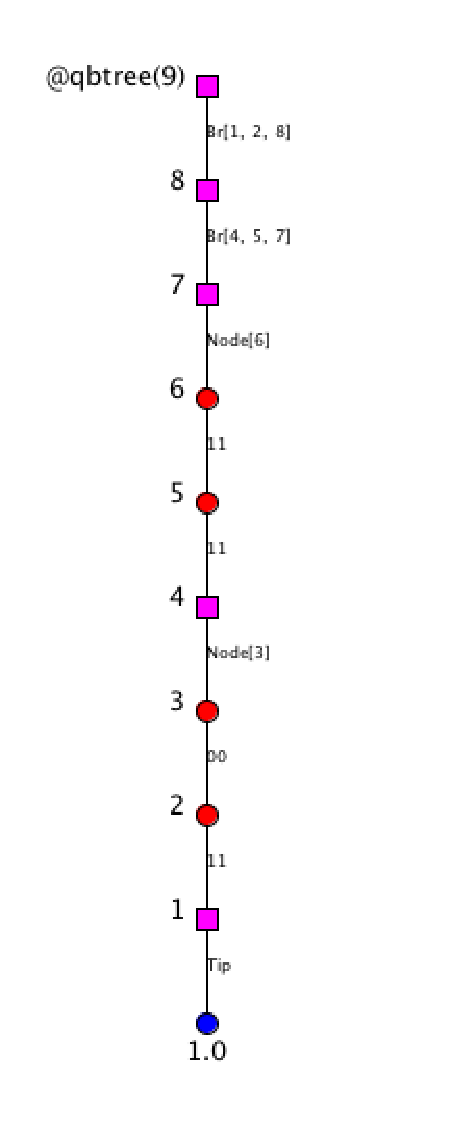
\includegraphics[scale=.5]{images/treeExampleInQSTrimmed.eps}}
\end{center}
\caption{Quantum stack contents after creation of \inlqpl{qbtree}}\label{fig:treeExampleInQS}
\end{figure}
The assignment statement which creates \inlqpl{qbtree} uses five constructor
expressions. The second assignment statement, which creates
\inlqpl{intlist} uses six constructor expressions and one function expression.
% The extent of the constructor expressions are shown by the underlines here.
% {\begin{multline*}\footnotesize
%\shoveleft{\mathtt{qbtree =}
%\underline{\mathtt{Br(}\underline{\mathtt{Tip}}\mathtt{,\ket{1},}
%\underline{\mathtt{Br(}\underline{\mathtt{Node(\ket{0})}}
%\mathtt{,\ket{1},}
%\underline{\mathtt{Node(\ket{1})}})})}; }\\
%\shoveleft{\mathtt{intlist =}
%\mathtt{reverse(}\underline{\mathtt{Cons(5,}
%\underline{\mathtt{Cons(4,}
%\underline{\mathtt{Cons(3,}
%\underline{\mathtt{Cons(2,}
%\underline{\mathtt{Cons(1,}
%\underline{\mathtt{Nil}}\mathtt{)}}\mathtt{)}}\mathtt{)}}\mathtt{)}}\mathtt{)}}\mathtt{)};}
%\end{multline*}
% }

Constructor expressions either have no arguments
 (e.g. \inlqpl{Tip}, \inlqpl{Nil} above), or
require a parenthesized list of expressions which agree in both
number and type with the template supplied at the declaration of the
type. These expressions are unrestricted otherwise. They may be constants,
identifiers, other constructor expressions, expression calls or compound
expressions. Any expressions that are classical in nature, such as constants,
are upgraded to quantum automatically.

\subsection{Function expressions}\label{subsec:expressioncalls}
When a function returns a single value, it may be used in a
function expression. The bottom two lines of listing below shows
two examples of function expressions.
\begin{lstlisting}[style=linqpl]
      f::(c1:Int, c2:Int, c3:Int | q1:Qubit, i1:Int ; out:Qubit)
      = { ... }
      ...
         qout  = f(c1,c2,c3 | q1,i2);
   qlist = Cons(f(1,2,3 | qout,5),Nil);
\end{lstlisting}
In the first function expression, \inlqpl{f} is the right hand side of
an assignment statement. The assignment statement
 creates the variable \inlqpl{qout}
with the value returned by the function.

In the second function expression, \inlqpl{f} is the first argument of a
constructor expression which will create a one element \inlqpl{List(Qubit)}.
The constructor expression is part of an assignment statement which
creates the variable \inlqpl{qlist} and sets it to
the one element list. Note that due to linearity, the variable
\inlqpl{qout} is no longer available after the second function expression.

A function expression is always a quantum expression, so it may only be
used in those places where quantum expressions are allowed. Nesting of
these calls inside constructor expressions, other function expressions
and function calls is allowed.

\begin{figure}[htbp]
\lstinputlisting[style=linqpl]{examplecode/append.qpl}
\caption{\lqpl{} code for appending two lists}\label{fig:appendtwolists}
\end{figure}

In \vref{fig:appendtwolists}, line \ref{line:append:funcexp} shows the
\inlqpl{append} being used as a function expression inside of a
constructor expression.

\chapter{BNF description of  the Linear Quantum Programming Language}\label{chap:formalSpecificationLinearQuantumProgrammingLanguage}
\section{Program definition}\label{sec:bnfProgramDefinition}
\lqpl{} programs consist of a series of definitions at the
global level. These are either \emph{data definitions} which
give a description of an algebraic data type \emph{procedure definitions}
which define executable code.

\begin{singlespace}
\begin{bnf}
   <Linearqplprogram>   :: <global definitions>
  
   <global_definitions> :: <global_definitions> <global_definition>
        | empty 
  
   <global_definition> :: <data_definition>
        | <procedure_definition>
\end{bnf}
\end{singlespace}

\section{Data definition}\label{sec:bnfDataDefinition}
A data definition consists of declaring a type name, with an optional
list of type variables and a list of constructors for that type. 
It is a semantic error to have different types having the same 
constructor name, or to redeclare a type name. 

Constructor definitions allow either fixed types or uses of the
type variables mentioned in the type declaration. 

\begin{singlespace}
\begin{bnf}
   <data_definition> :: <type_definition> '=' 
                        '\{' <constructor_list> '\}'
  
   <type_definition> :: 'type' <constructorid> <id_list>
  
   <constructor_list>:: <constructor> <more_constructor_list>
      
   <more_constructor_list> :: 
        '|' <constructor> <more_constructor_list>
        | \{- empty -\}
  
   <constructor> :: <constructorid> '(' <typevar_list> ')'
        | <constructorid>
  
   <typevar_list> :: <typevar> <moretypevar_list>
             
   <moretypevar_list> :: ',' typevar moretypevar_list
        | \{- empty -\} 

   <typevar> :: <identifier> 
        | <identifier>
        | <constructor>
        | <constructor> '(' <typevar_list> ')' 
        | <builtintype>

   <builtintype>:: 'Qubit'  | 'Int' | 'Bool'
\end{bnf}
\end{singlespace}

\section{Procedure definition}\label{sec:bnfProcedureDefinition}
Procedures may only be defined at  the global level
in a \lqpl{} program. The definition consists of
a procedure name, its input and output formal parameters and
a body of code. Note that a procedure may have either no input, no
outputs or neither.

The classical and quantum inputs are  separated by a '|'. 
Definitions with either no parameters or no classical parameters are
specific special cases. 

\begin{singlespace}
\begin{bnf}
   <procedure_definition> :: <identifier> '::' 
            '(' <parameter_definitions> '|' 
	        <parameter_definitions> ';' 	
                <parameter_definitions>  ')'
                    '='  <block>
        | <identifier> '::' 
            '(' <parameter_definitions> ';' 	
                <parameter_definitions>  ')'
                    '='  <block>
        | <identifier> '::' '(' ')' '=' <block>
  
   <parameter_definitions> :: <parameter_definition>
             <more_parameter_definitions>
        | \{- empty -\}
  
   <more_parameter_definitions> :: ',' <parameter_definition> 
	     <more_parameter_definitions>
        | \{- empty -\}
  
   <parameter_definition> :: <identifier> ':' <constructorid>
             '(' <typevar_list> ')' 
        | <identifier> ':' <constructorid>
        | <identifier> ':' <builtintype>
     
\end{bnf}
\end{singlespace}

\section{Statements}\label{sec:bnfStatementDefinition}
Although \lqpl{} is a functional  language, the language retains the
concept of \emph{statements} which provide an execution flow for the
program. 

The valid collections of statements are \emph{blocks} which
are lists of statements.

\begin{singlespace}
\begin{bnf}   

   <block> :: '\{' <stmtlist> '\}' 
  
   <stmtlist>:: <stmtlist> ';' <stmt>
        | <stmtlist> ';'
        | <stmt>
        | \{- empty -\}
     
\end{bnf}
\end{singlespace}

Statements are broadly grouped into a few classes.
\subsection{Assignment} 
Variables are created by assigning to them. There is no 
ability to separately declare them. Type unification will determine the
appropriate type for the variable.

\begin{singlespace}
\begin{bnf}   
   <stmt> :: <identifier> '=' <exp>
\end{bnf}
\end{singlespace}

\subsection{Case statements} 
These are \inlqpl{measure, case, use, discard} and
the classical assign, \inlqpl{:=}. 
These statements give the programmer the capability to
specify different processing on the sub-stacks of
a quantum variable. This is done with dependant statements. 
For  \inlqpl{measure} 
and \inlqpl{case},
the dependent statements are in the block specified in the 
statement. For \inlqpl{use}, they may be
specified explicitly, or they may be all the 
statements following the \inlqpl{use} to the end
of the enclosing block. The classical assign is syntactic sugar for an
assignment followed by a \inlqpl{use} with no explicit dependent statements.

The \inlqpl{discard} statement is grouped here due to the quantum effects.
Doing a discard of a \qubit{} is equivalent to measuring the \qubit{} and 
ignoring the results. This same pattern is followed for discarding 
quantum variables of all types.

\begin{singlespace}
\begin{bnf} 
   (<stmt> continued)    
        | 'case' <exp> 'of' <cases>  
        | 'measure' <exp> 'of' <zeroalt> <onealt> 
	| <identifier> ':=' <exp>
        | 'use' <identifier_list> <block>
        | 'use' <identifier_list> 
\end{bnf}
\end{singlespace}

\subsection{Functions} 
This category includes procedures and
transforms. A variety of calling syntax is available, however, there
are no semantic differences between them.

\begin{singlespace}
\begin{bnf}   
   (<stmt> continued)  
        | '(' <identifier_list> ') '=' 
	      <callable>  '(' <exp_list> ')'
        | '(' <identifier_list> ') '='
	      <callable>  '(' <exp_list> '|' <exp_list> ')'
        | <callable> <ids>
        | <callable> '(' <exp_list> ')' <ids>
        | <callable> '(' <exp_list> '|' <exp_list> ';' 
	      <ids> ')'
\end{bnf}
\end{singlespace}

\subsection{Blocks} 
The block statement allows grouping of a 
series of statements by enclosing them with \inlqpl{\{} and \inlqpl{\}}.
An empty statement is also valid.

\begin{singlespace}
\begin{bnf}   
   (<stmt> continued)  
        |  <block>  
	| \{- empty -\}  
\end{bnf}
\end{singlespace}

\subsection{Control} 
\lqpl{} provides a statement for classical control and
one for quantum control. Note that quantum control affects only the semantics
of any transformations applied within the control. Classical control requires
the expressions in its guards (see below) to be classical and not quantum.

\begin{singlespace}
\begin{bnf}   
   (<stmt> continued)  
        | 'if' guards
	| <stmt> '<=' <control_list>
\end{bnf}
\end{singlespace}

\subsection{Divergence}
 This signifies that this portion of the program does not
terminate. Statements after this will have no effect. 
\begin{singlespace}
\begin{bnf}   
   (<stmt> continued)  
        | 'zero'                       
\end{bnf}
\end{singlespace}

\section{Parts of statements}\label{sec:bnfStatementPartsDefinition}
The portions of statements are explained below. First is
\emph{callable} which can be either a procedure name or a 
particular unitary transformation.

\begin{singlespace}
\begin{bnf}  
   <callable> :: <identifer> | <transform>
\end{bnf}
\end{singlespace}

The alternatives of a measure statement consist of choice indicators 
for the base of the measure followed by a block of statements.

\begin{singlespace}
\begin{bnf} 
   <zeroalt> ::  '|0>' '=>' <block>
  
   <onealt> :: '|1>' '=>' <block>
\end{bnf}
\end{singlespace}

The \inlqpl{if} statement requires a list of \emph{guards} following it.
Each guard is composed of a  classical expression that will evaluate to 
\inlqpl{true} or \inlqpl{false}, followed by a block of guarded statements. 
The statements guarded by the expression will be executed only when
the expression in the guard is true. 
The list of guards must end with a  default guard
called \inlqpl{else}. Semantically, this is equivalent to putting a guard of
\inlqpl{true}.

\begin{singlespace}
\begin{bnf} 
   <guards> :: <freeguards> <owguard>

   <freeguards> :: <freeguard> <freeguards>
        | \{- empty -\}

   <freeguard> :: <exp> '=>' <block>

   <owguard> :: 'else' '=>' <block>
\end{bnf}
\end{singlespace}

When deconstructing a data type with a \inlqpl{case} statement, a
pattern match is used to determine which set of dependent 
 statements are executed. The patterns allow the programmer
to either throw away the data element (using the '\inlqpl{\_}' special 
pattern), or assign it to a new identifier.

\begin{singlespace}
\begin{bnf}   
   <cases> :: <case> <more_cases> 
  
   <more_cases> :: \{- empty -\}
        | <case> <more_cases>
  
   <case> :: <caseclause> '=>' <block>
  
   <caseclause> ::  <constructorid> '(' <pattern_list> ')' 
        | <constructorid>
  
   <pattern_list>:: <pattern> <more_patterns>

   <more_patterns> :: ',' <pattern> <more_patterns>
        | \{- empty -\} 

   <pattern> :: <identifier> | '_'
\end{bnf}
\end{singlespace}

\section{Expressions}\label{sec:bnfExpressionDefinition}
\lqpl{} provides  standard expressions, with the restriction that
 arithmetic expressions 
 may be done only on classical values. That is, they must be 
on the classical stack or a constant.

The results of comparisons are Boolean values that will be held on
the classical stack.

\begin{singlespace}
\begin{bnf}   

   <exp>:: <exp0> 
  
   <exp0>:: <exp0> <or_op> <exp1> | <exp1>
  
   <exp1>:: <exp1> '&&' <exp2> | <exp2> 
  
   <exp2>:: '~' <exp2> | <exp3>  | <exp3> <compare_op> <exp3>
  
   <exp3>:: <exp3> <add_op> <exp4> | <exp4>
  
   <exp4>:: <exp4> <mul_op> <exp5> | <exp5> 
  
   <exp5>:: <exp5> <shift_op> <exp6> | <exp6>
  
   <exp6>:: <identifier> | <number> | 'true' | 'false' 
        | '(' <exp> ')' 
        | <constructorid> '(' <exp_list> ')' 
        | <constructorid>
	| <identifier> '('  ')'
        | <identifier> '(' <exp_list> ')'  
        | <identifier> '(' <exp_list> ';' ids ')'
	| '|0>' | '|1>'
  
   <exp_list>:: <exp> <more_exp_list>
  
   <more_exp_list>:: ',' <exp> <more_exp_list>  
        | \{- empty -\} 
\end{bnf}
\end{singlespace}

\section{Miscellaneous and lexical}\label{sec:bnfMiscLexicalDefinition}
These are the basic elements of the language as used above. Many of these
items are differentiated at the lexing stage of the compiler.

\begin{singlespace}
\begin{bnf}   

   <idlist> :: <identifier> more_ids
        | \{- empty -\}
 
   <more_ids> :: <identifier> more_ids
        | \{- empty -\}
 
   <control_list>:: <control> <more_control_list>

   <more_control_list>:: ',' <control> <more_control_list>
        | \{- empty -\}
  
   <control>:: <identifer>   | '~' <identifer>

   <opt_identifier_list>:: <identifier_list>
        | \{- empty -\}
        
   <identifier_list>:: <identifier> <more_idlist>

   <more_idlist>:: ',' <identifier> <more_idlist> 
        | \{- empty -\}
  
   <or_op>:: '||' | '^'
  
   <compare_op>:: '==' | '<' | '>' | '=<' | '>=' | '=/=' 

   <add_op>::'+' | '-' 

   <mul_op>::'*' | 'div'  | 'rem'

   <shift_op>::'>>' | '<<'

   <transform>:: <gate> 
        | <transform> *o* transform 

   <gate> :: 'Had' | 'T'  | 'Phase' | 'Not' |  'RhoX'  
	| 'Swap' | 'Rot '| 'RhoY ' | '  RhoZ ' | 'Inv-'<gate>

   <identifier> :: <lower> | <identifier><letterOrDigit>
   <constructorid :: <upper> | <constructorid><letterOrDigit>
   <letterOrDigit> :: <upper>|<lower>|<digit>
   <number> :: ['+'|'-'] <digit>+
   <lower> ::   'a' | 'b' | 'c' | 'd' | 'e' | 'f' | 'g' 
        | 'h' | 'i' | 'j' | 'k' | 'l' | 'm' | 'n' | 'o' 
        | 'p' | 'q' | 'r' | 's' | 't' | 'u' | 'v' | 'w' 
	| 'x' | 'y' | 'z'
   <upper> ::   'A' | 'B' | 'C' | 'D' | 'E' | 'F' | 'G' 
        | 'H' | 'I' | 'J' | 'K' | 'L' | 'M' | 'N' | 'O' 
        | 'P' | 'Q' | 'R' | 'S' | 'T' | 'U' | 'V' | 'W' 
        | 'X' | 'Y' | 'Z'
   <digit> ::   '0' | '1' | '2' | '3' | '4' | '5' | '6' 
        | '7' | '8' | '9'
\end{bnf}
\end{singlespace}

\chapter{Quantum stack machine additional details}\label{chap:qsmadditional}
\section{Instructions}\label{subsec:repauxinstructions}
Creation of reasonable set of instructions, balancing brevity and usefulness
has been an interesting task. The list of instructions and brief
descriptions of them are presented in \vref{tab:instructionlist}. The 
transitions of these are presented formally 
in \vref{sec:stackmachineoperation}.

{\begin{singlespace}
\tablecaption{QSM instruction list}\label{tab:instructionlist}
\tablehead{\hline \textbf{Instruction}&\textbf{Arguments}&\textbf{Description}\\ \hline}
\tabletail{\hline \multicolumn{3}{r}{\emph{Continued on next page}}\\}
\tablelasttail{\hline}
\begin{supertabular}{|p{.85in}|p{1.2in}|p{3.69in}|}
\qsmins{QLoad}&\emph{nm:Name}, \emph{k::\qubit}&Creates \qubit{} named \emph{nm}
 and sets the value to \ket{k}.\\ & & \\
\qsmins{QMove}&\emph{nm:Name} &Creates an integer or Boolean named \emph{nm}
 and sets its value to the top of the classical stack.\\ & & \\
\qsmins{QCons}&\emph{nm:Name}, \emph{c::constructor} &Creates a data type element
with the value \emph{c}. Note that if the constructor requires sub-elements,
this will need to be followed by \qsmins{QBind} instructions.\\ & & \\
\qsmins{QBind}&\emph{nm:Name}&Binds the node $[nm]$ to 
the data element currently on 
the top of the stack.\\
\hline
\qsmins{QDelete}&$\emptyset$&Deletes the top node and any
 bound nodes in the quantum stack.\\ & & \\
\qsmins{QDiscard}&$\emptyset$&Discards the node on top of
 the quantum stack.\\ & & \\
\qsmins{QUnbind}&\emph{nm:Name}&Unbinds the first bound node 
from the data element at
the top of the stack and assigns it as \emph{nm}.\\ 
\hline
\qsmins{QPullup}&\emph{nm::name}&Pulls the node named 
\emph{nm} to the top of the 
quantum stack.\\ & & \\
\qsmins{QName}&\emph{nm1::name}, \emph{nm2::name}&Renames 
the node named \emph{nm1} to 
\emph{nm2}.\\
\hline
\qsmins{AddCtrl}&$\emptyset$&Marks  the start
of a control point in the control stack. Any following \qsmins{QCtrl} 
instructions will add the top node to this control point.\\ & & \\
\qsmins{QCtrl}&$\emptyset$&Moves the top element of the quantum stack
to the control stack. Recursively moves any bound nodes to the control
stack when the element is 
a constructed data type.\\ & & \\
\qsmins{UnCtrl}&$\emptyset$&Moves all items in the  control stack at the
current control point back to the quantum stack.\\ & & \\
\qsmins{QApply}&\emph{i::Int},\emph{t:Transform}&Parametrizes the transform \emph{T} with
the top \emph{i} elements of the classical stack and applies it to the
 quantum stack.\\
\hline
\qsmins{Measure}&\emph{l0::Label}, \emph{l1::Label}&Measures 
the \qubit{} on top of the
quantum stack and sets up the dump for execution of
 the code at \emph{l0} for the $00$ sub-branch and 
the code at \emph{l1} for the $11$ sub-branch.\\ & & \\
\qsmins{Split}&\emph{cls::[(constructor, Label)]}&Splits the data node at 
the top of the
quantum stack and sets up the dump  for execution of the code at 
the $i$-th label for the $i$-th  sub-branch.\\ & & \\
\qsmins{Use}&\emph{lbl::Label}&Uses the classical 
(integer or Boolean) node on top of the
quantum stack and sets up the dump to for execution of the code at 
\emph{lbl} for each of the sub-branches.\\ & & \\
\qsmins{SwapD}&$\emptyset$&Merges the current quantum stack
 with the results stack of the
dump, activates the next partial stack to be processed
 and jumps to the code at the corresponding 
label. When there are no more partial stacks, the instruction 
merges the current
stack with the the results stack and sets that as the new quantum stack.\\
\hline
\qsmins{Call}&\emph{i::Int}, \emph{ep::EntryPoint}&For the first element of the 
infinite list of states, sets the values at the leaves of the 
quantum stack to $0$. 
For the remainder of the list, the instruction jumps to the 
subroutine at \emph{ep}, saving
the return location and classical stack on the dump. It copies the
top \emph{i} elements of the classical stack for the subroutine.\\ & & \\
\qsmins{Return}&\emph{i::Int}&Restores the location and classical stack from the
dump, copies the top \emph{i} items of the current classical stack to the
top of the restored classical stack.\\
\hline
\qsmins{Jump}&\emph{lbl::Label}&Jumps \emph{forward} to the label \emph{lbl}.\\ & & \\
\qsmins{CondJump}&\emph{lbl::Label}&If the top of the classical stack is the
value \terminalio{false}, jumps \emph{forward} to the label \emph{lbl}.\\ & & \\
\qsmins{NoOp}&$\emptyset$&Does nothing.\\
\hline
\qsmins{CGet}&\emph{i::Int}&Copies the \emph{i}-th element of the 
classical stack to the
top of the classical stack. A negative value for \emph{i} indicates the
instruction should copy the $|i|^{\text{th}}$ value from the
bottom of the classical stack.\\ & & \\
\qsmins{CPut}&\emph{i::Int}&Copies the top of the classical stack to the 
\emph{i}-th element of the classical stack.  A negative value for 
\emph{i} indicates the
instruction should place the value into the $|i|^{\text{th}}$ location
 from the
bottom of the classical stack.\\ & & \\
\qsmins{CPop}&$\emptyset$&Pops off (and discards) the top element of 
the classical stack.\\ & & \\
\qsmins{CLoad}&\emph{v::Either Int Bool}&Pushes \emph{v} onto the classical stack.\\ & & \\
\qsmins{CApply}&\emph{op::Classical Op}&Applies \emph{op} to the top elements of
the classical stack, replacing them with the result of the operation.\\
\end{supertabular}
\end{singlespace}
}

\section{Translation of \lqpl{} to stack machine code}\label{sec:translationtoqsmcode}
This section will discuss the code produced by the 
various statements and expressions in an \lqpl{} program.
An \lqpl{} program consists of
a collection of data definitions and procedures. Data definitions do not
generate any direct code but do affect the code generation of statements
and expressions.

Each procedure will generate code. A procedure consists of a collection of
statements each of which will generate code. Some statements may have other
statements of expressions as dependent pieces, which again will generate 
code.

The code generation in the compiler, and the description here, follows a
standard recursive descent method.
\subsection{Code generation of procedures}\label{subsec:cgprocedures}

The code generated for each procedure follows a standard pattern of: 
procedure entry; procedure statements; procedure exit. The procedure statements 
portion is the code generated for the list of statements of the procedure, each of
which is detailed in \vref{subsec:cgstatements}.

\subsubsection{Procedure entry}
Each procedure is identified in QSM by an entry point, using an assembler directive.
This directive is a mangled name of the procedure, followed by the keyword 
\qsmins{Start}. The only exception to this is the special procedure 
\qsmins{main} which is generated without mangling. \qsmins{main} is always
the starting entry point for a QSM program.

\subsubsection{Procedure exit}
The end of all procedures is denoted by another assembler directive, 
\qsmins{EndProc}. For all procedures except \qsmins{main}, the code generation
determines how many classical variables are being returned by the procedure
and emits a \qsmins{Return} $n$ instruction, where $n$ is that count\footnote{This
functionality is currently not available in \lqpl{}, but may be re-introduced at
a later date.}.

\subsubsection{Procedure body}
The code for each statement in the list of statements is generated and used as the 
body of the procedure.
\begin{figure}[htbp]
\centering
\subfloat[Coin flip code]{
\begin{singlespace}
\lstinputlisting[style=linqpl]{examplecode/coinnolbls.qpl}
\end{singlespace}}\qquad
\subfloat[Generated  code]{
\begin{singlespace}
\lstinputlisting[style=linqpl]{examplecode/coin.generated}
%VerbatimInput[numbers=left,numbersep=3pt]{examplecode/coin.generated}
\end{singlespace}
}
\caption{\lqpl{} and QSM coin flip programs}\label{fig:cg:coin}
\end{figure}
As an example, see the coin flip code and the corresponding generated QSM code
in \vref{fig:cg:coin}.

\subsection{Code generation of statements}\label{subsec:cgstatements}
Each statement in \lqpl{} generates code. The details of the
code generation for each statement are given in the following pages, together
with examples of actual generated code.
\subsubsection{Assignment statements}
The sub-section describes code generation for quantum assignment statements and
assignments to variables on the classical stack. The classical assignment ($:=$)
statement is described with the \inlqpl{use} statement below, as it is
syntactic sugar for that statement.

An assignment of the form $i = \langle expr \rangle$ is actually 
broken down into 5 special cases. The first is when the left hand side is
an in-scope variable that is on the classical stack. The other four all 
deal with the case of a quantum variable, which is either introduced or
overwritten. The four cases depend on the type of expression on the 
right hand side. Each paragraph  below will identify which case is
being considered and then describe the code generation for that case.

\paragraph{Left hand side is a classical variable.} In this case, generate
the code for the expression on the right hand side (which will be classical
in nature). This leaves the expression value at the top of the classical
stack. Now, emit a \qsmins{CPut} instruction which will copy that value
into the location of the classical variable.

\begin{center}
\begin{tabular}{p{1in}p{.5in}p{1.5in}}
{\begin{singlespace}
\begin{lstlisting}[style=linqpl]
i = 5;
\end{lstlisting}
\end{singlespace}}
 & { \quad \quad \raisebox{.8em}{$\implies$}} &
{\begin{singlespace}
\begin{lstlisting}[style=linqpl]
     CLoad 5
     CPut -2
\end{lstlisting}
\end{singlespace}}
\end{tabular}
\end{center}


\paragraph{Right hand side is a classical expression.} First, generate the
expression code, which leaves the value on the top of the classical stack.
Then emit a \qsmins{QMove} instruction with the name of the left hand side.
This will create a new classical node, which will be set to the value of the
top of the classical stack.


\begin{center}
\begin{tabular}{p{1in}p{.5in}p{1.5in}}
{\begin{singlespace}
\begin{lstlisting}[style=linqpl]
i = 5;
\end{lstlisting}
\end{singlespace}}
 & { \quad \quad \raisebox{.8em}{$\implies$}} &
{\begin{singlespace}
\begin{lstlisting}[style=linqpl]
     CLoad 5
     QMove i
\end{lstlisting}
\end{singlespace}}
\end{tabular}
\end{center}


\paragraph{Right hand side is a constant \qubit.} Emit the 
\qsmins{QLoad} instruction  with the \qubit{} value and the left hand side
variable name.

\begin{center}
\begin{tabular}{p{1in}p{.4in}p{1.5in}}
{\begin{singlespace}
\begin{lstlisting}[style=linqpl]
q = |1>;
\end{lstlisting}
\end{singlespace}}
 & { \raisebox{-1.3em}{$\implies$}} &
{\begin{singlespace}
\begin{lstlisting}[style=linqpl]
     QLoad q |1>
\end{lstlisting}
\end{singlespace}}
\end{tabular}
\end{center}


\paragraph{Right hand side is an expression call.}
First, emit the code for the expression call. This will leave the
result quantum value on the top of the quantum stack. If the
formal name given by the procedure definition is the same as the
left hand side name, do nothing else, as the variable is already
created with the proper name. If not, emit a \qsmins{QName} instruction
to rename the last formal parameter name to the left hand side name.

\begin{center}
\begin{tabular}{p{2in}p{.3in}p{1.75in}}
{\begin{singlespace}
\begin{lstlisting}[style=linqpl]
random :: (maxval :Int; 
       rand :Int) = {...}
...
x = random(15);
\end{lstlisting}
\end{singlespace}}
 & { \qquad \qquad \quad \quad \qquad \qquad $\implies$} &
{\begin{singlespace}
\begin{lstlisting}[style=linqpl]
CLoad 15
QMove c18
QName c18 maxval //In
Call 0 random_fcdlbl0
QName rand x //Out
\end{lstlisting}
\end{singlespace}}
\end{tabular}
\end{center}


\paragraph{Right hand side is some other expression.}
Generate the code for the expression. Check the name on the top of
the stack. If it is the same as the left hand side name, do nothing else,
otherwise emit a \qsmins{QName} instruction.


\begin{center}
\begin{tabular}{p{2in}p{.3in}p{1.5in}}
{\begin{singlespace}
\begin{lstlisting}[style=linqpl]
outqs = Cons(q, inqs');
\end{lstlisting}
\end{singlespace}}
 & { \qquad \qquad \quad \quad \qquad \qquad $\implies$} &
{\begin{singlespace}
\begin{lstlisting}[style=linqpl]
    QCons c4 #Cons
    QBind inqs'
    QBind q
    QName c4 outqs
\end{lstlisting}
\end{singlespace}}
\end{tabular}
\end{center}


\subsubsection{Measurement code generation}
%FIXME
% We *should* be able to get away with, yes, m0, m1 and mf, but no spurious
% EndQC(now swap) statement.
Measurement will always have two subordinate sets of statements,
respectively for the \ket{0} and \ket{1} cases. 
The generation for the actual statement will handle the requisite branching.

The code generation first acquires three new labels, $m_0,m_1$ and $m_f$. It
will then emit a \qsmins{Measure}~$m_0\ m_1$ statement, followed by 
a \qsmins{Jump}~$m_f$. Recall from the transitions 
in \vref{subsec:transitiondiagrams} that when the machine executes
the \qsmins{Measure} instruction, \emph{it then generates and executes a}
\qsmins{SwapD} instruction. The \qsmins{Jump} will be executed when 
all branches of the \qubit{} have been executed.

Then, for each of the two sub blocks ($i\in\{0,1\}$), 
I emit a \qsmins{Discard} labelled with $m_i$. This is followed by the 
code generated from the corresponding block of statements. Finally a 
\qsmins{SwapD} is emitted.

The last instruction generated is a \qsmins{NoOp} which is labelled
with $m_f$.


\begin{center}
\begin{tabular}{p{2in}p{.3in}p{1.5in}}
{\begin{singlespace}
\begin{lstlisting}[style=linqpl]
measure q of 
 |0> => {n1 = 0}
 |1> => {n1 = 1};
\end{lstlisting}
\end{singlespace}}
 & { \qquad \qquad \quad \quad \qquad \qquad $\implies$} &
{\begin{singlespace}
\begin{lstlisting}[style=linqpl]
   QPullup q
   Measure l7 l8
   Jump l9
l7 QDiscard
   CLoad 0
   QMove n1
   SwapD
l8 QDiscard
   CLoad 1
   QMove n1
   SwapD 
l9 NoOp
\end{lstlisting}
\end{singlespace}}
\end{tabular}
\end{center}


\subsubsection{Case statement code generation}

Case statement generation is conceptually similar to that of
measurement. The  differences are primarily due to the variable 
number of case clauses and the need to instantiate the variables of the 
patterns on the case clauses.

As before, the expression will have its code generated first.
Then, the compiler will use a function to return a list of triples of
a constructor, its generated label and the corresponding code for
 each of the case clauses. 
The code generation done by that function is detailed below.

At this point, the code generation resembles measurement generation.
The compiler generates a label $c_f$ and emits
a \qsmins{Split} with a list of constructor / code label pairs which
have been returned by 
the case clause generation. This is followed by emitting
a \qsmins{Jump}~$c_f$. 
After the \qsmins{Jump} has been emitted, 
the code generated by the case clause generation is emitted.

The final instruction generated is a \qsmins{NoOp} which is labelled
with $c_f$.

\paragraph{Case clause code generation.} 
The code generation for a case clause has a rather complex prologue which
ensures the assignment of any bound variables to the patterns in the 
clause.

First, the code generator gets
 a new label $c_l$ and then calculates the unbinding code as follows:
For each \emph{don't care} pattern in the clause, code is 
generated to delete the corresponding bound node. 
This is done by first getting a new stack name $nm$, then
adding the instructions \qsmins{QUnbind}~$nm$, \qsmins{Pullup}~$nm$ and
\qsmins{QDelete}~$nm$. This accomplishes the unbinding of that node and
removes it from the quantum stack. Note that \qsmins{QDelete} is used here
to ensure that all subordinate nodes are removed and that no spurious data
is added to the classical stack in the case of the don't care node being a
classical value.

For each  named pattern $p$, only the
instruction \qsmins{QUnbind}~$p$ is added.

The program now has a list of instructions that will accomplish unbinding
of the variables. Note this list may be empty, e.g., the \inlqpl{Nil}
constructor for \inlqpl{List}.

The clause generation now creates its own return list. When the 
unbinding list is not empty, these instructions are added first, with
the first one of them being labelled with $c_l$.This is followed by
a \qsmins{Discard} which discards the decomposed data node. 
When the unbind list  is
empty, the first instruction is the \qsmins{Discard} labelled by $c_l$.

Then, the code generated by the statements in the case clause block are
added to the list. Finally, a \qsmins{SwapD} is added at the end.

The lists from all the case clauses are combined and this is returned to the
case code generation.

The example at the end of the use clause will illustrate both the case clause 
and the use statement code generation.

\subsubsection{Use and classical assign code generation}
As described earlier in \vref{subsec:usestatements}, the classical assignment, 
\inlqpl{v := exp} is syntactic sugar for a variable assignment followed by
a \inlqpl{use} statement. The code generation for each is 
handled the same way.

There are two different cases to consider when generating this code.
 The \inlqpl{use} statement
may or may not have subordinate statements. In the case where it does not have
any subordinate statements, (a classical assign or a
 use with no block), the scope
of the classical variables in the use 
extends to the end of the enclosing block.

The case  of a use with a subordinate block  is presented first.

\paragraph{Use with subordinate block code generation.}
While similar to the generation for the measure and case statements,
there are differences. The two main differences are that there is only one
subordinate body of statements and that  multiple variables may be
used.

In the case where there is a single use variable $nu$, the generator gets
the body label $u_b$ and end label $u_e$. It then emits a 
\qsmins{Pullup}~$nu$, a \qsmins{Use}~$u_b$ and a \qsmins{Jump}~$u_e$.
This is followed by emitting
 a \qsmins{Discard} labelled by $u_b$ and the code generated
by the subordinate body of statements and a \qsmins{SwapD} instruction.
This is terminated by a \qsmins{NoOp} labelled by $u_e$.

When there are multiple names $n_1,n_2,\ldots,n_j$, the generator first
recursively generates code assuming the same body of 
statements but with a use statement that only has the variables 
$n_2,\ldots,n_j$. This is then used as the body of code for
a use statement with only one variable $n_1$, which is generated
in the same manner as in the above paragraph.

\paragraph{Use with no subordinate block.}
To properly generate the code for this, including the \qsmins{SwapD} and
end label, the generator uses
 the concept of delayed code. The prologue (\qsmins{Use},
\qsmins{Jump} and \qsmins{Discard}) and epilogue (\qsmins{SwapD}, \qsmins{NoOp})
are created in the same manner as the use with the subordinate block.
The prologue is emitted at the time of its generation. The epilogue, however,
is added to a push-down stack of delayed code which is emitted at the
end of a block.  See the description of the block code generation for more
details on this. These items are illustrated in \vref{fig:gencasecode}.

\begin{figure}[htbp]
\begin{center}
\begin{tabular}{p{2in}p{.3in}p{2.5in}}
{\begin{singlespace}
\begin{lstlisting}[style=linqpl]
case l of
  Nil => {i = 0}
  Cons (_, l1) => {
    n= len(l1);
    use n;
    i = 1 + n;
}
\end{lstlisting}
\end{singlespace}}
 & { \qquad \qquad \quad \quad \qquad \qquad $\implies$} &
{\begin{singlespace}
\begin{lstlisting}[style=linqpl]
 Split (#Nil,l0) (#Cons,l1) 
   Jump l4
l0 QDiscard
   CLoad 0
   QMove i
   SwapD
l1 QUnbind c0
   QUnbind l1
   QDiscard
   QPullup c0
   QDiscard 
   QPullup l1
   QName l1 l
   Call 0 len_fcdl0
   QName i n
   QPullup n
   Use l2
   Jump l3
l2 QDiscard 
   CLoad 1
   CGet 0
   CApply +
   QMove i
   SwapD //For Use
l3 NoOp
    SwapD //For Split
l4 NoOp
\end{lstlisting}
\end{singlespace}}
\end{tabular}
\end{center}
\caption{QSM code generated for a case and use statement.}\label{fig:gencasecode}
\end{figure}



\subsubsection{Conditional statements}
The \inlqpl{if ... else} statement allows the programmer to specify an
unlimited number of classical expressions to control blocks of code. Typically,
this is done within a \inlqpl{use} statement based upon the variables used.

The statement code generation is done by first requesting a new label, $g_e$.
This label is used in the next step,  generating the 
code for all of the guard clauses. The generation is completed by emitting a 
\qsmins{NoOp} instruction labelled by $g_e$.

\paragraph{Guard clauses.}\label{para:guardclauses} 
Each guard clause consists of an expression and
list of statements. The code generator first emits
 the code to evaluate the expression. 
Then, a new label $g_l$ is requested and the instruction \qsmins{CondJump}~$g_l$
is emitted. The subordinate statements are generated and emitted, 
considering them as a 
single block. The concluding instruction is a \qsmins{Jump}~$g_e$.

At this point, if there are no more guard clauses, a \qsmins{NoOp} instruction,
labelled by $g_l$ is emitted, otherwise the code generated by the remaining
guard clauses is labelled by $g_l$ and emitted.
%FIXME - check that this is right and what really happens - appears that
% multiple branches would not be right...

\begin{center}
\begin{tabular}{p{2in}p{.3in}p{2.5in}}
{\begin{singlespace}
\begin{lstlisting}[style=linqpl]
if b == 0 => { 
   theGcd = a;
} else =>  { 
   (theGcd) = 
     gcd(b, a mod b);
}
\end{lstlisting}
\end{singlespace}}
 & { \qquad \qquad \quad \quad \qquad \qquad $\implies$} &
{\begin{singlespace}
\begin{lstlisting}[style=linqpl]
    CGet -2
    CLoad 0
    CApply ==
    CondJump lbl2
    CGet -1
    QMove theGcd
    Jump lbl1
lbl2 CLoad True //else
    CondJump lbl3
    CGet -1
    CGet -2
    CApply %
    QMove c0
    CGet -2
    QMove c1
    QName c1 a
    QName c0 b
    Call 0 gcd_fcdlbl0
    Jump lbl1
lbl3 NoOp
lbl1 NoOp
\end{lstlisting}
\end{singlespace}}
\end{tabular}
\end{center}


\subsubsection{Function calling and unitary transforms}\label{subsubsec:cgfunctioncalls}
The code generation of these two statements is practically the same, with
the only difference being that built in transformations have a special
instruction in QSM, while executing a defined function requires
the \qsmins{Call} instruction.

In each case, the statement allows for input classical and quantum expressions
and output quantum identifiers.

The first step is the generation of the code for the input 
classical expressions. These are generated in reverse order so that the 
first parameter is on the top of the classical stack, the second is next
and so forth. Then, the input quantum expressions are generated,
with names of these expressions being saved. Note that it is possible to use
expressions which are innately classical (e.g., constants and variables on
the classical stack) as a quantum expression. The compiler will generate 
the code needed to lift it to a quantum expression. See 
\vref{subsec:cglifting} for the details.

At this stage, the two
types differ slightly. For the unitary transformation case, the
code ``\qsmins{QApply}~$n$~!$t$'' is emitted, where $n$ is the number of 
classical arguments and $t$ is the name of the built in transform. The
exclamation mark is part of the QSM assembler syntax for transform names.
In a defined function, renames of the input quantum expressions to
the names of the input formal ids are generated, 
by emitting a series of \qsmins{QName} 
instructions. This is followed by emitting a \qsmins{Call}~$n$~$f$, 
where $n$ is again the number of classical arguments and $f$ is the 
internally generated name of the function.

In both cases, the code checks the formal return parameter names against
the list of return value names. For each one that is different, a 
\qsmins{QName}~$frml$~$retnm$ is emitted.

See the previous code list between the  \qsmins{CondJump lbl3} and
\qsmins{lbl3 NoOp} for an example of this.



\subsection{Code generation of expressions}\label{subsec:cgexpression}
In the previous sub-section, a number of examples of code generation
were given. These also illustrated most of the different aspects of 
expression code generation. A few additional examples are given below.

\subsubsection{Generation of constants}
There are three possible types of constants, a Boolean, an integer or 
a \qubit. Note that constructors are considered a different class of 
expression.

For both Boolean and integers, the compiler emits a \qsmins{CLoad}~$val$ 
instruction. For a \qubit, it creates a new name $q$ and emits
a \qsmins{QLoad}~$q$~$qbv$ instruction.

Examples of these may be seen in the sub-sub-section on assignments.

\subsubsection{Generation of classical arithmetic and Boolean expressions}
In all cases, these types of expressions are calculated solely on 
the classical stack. Whenever the generator encounters 
 an expression of the form
\[ e_1\ op\ e_2\]
it first emits the code to generate $e_2$, followed by the code to generate
$e_1$. This will leave the result of $e_1$ on top of the stack with $e_2$'s
value right below it. 
It then emits the instruction \qsmins{CApply}~$op$, which will
apply the operation to the two top elements, replacing them with the
result.

The Boolean \emph{not} operation is the only operation of arity 1. 
Code generation is done in the same manner. The generator emits code for the 
expression first, followed by \qsmins{CApply}~$\neg$.

 See  under Guard clauses, \vref{para:guardclauses} for
examples.

\subsubsection{Generation of variables}
The semantic analysis of the program will split this into two cases; 
classical variables and quantum variables. Each are handled differently.

\paragraph{Classical variables.} These variables are on the classical
stack at a specific offset. The use of them in an expression means 
that they are to be \emph{copied} to the top of the classical stack.
The code emitted is \qsmins{CGet}~$offset$, where $offset$ is the 
offset of the variable in the classical stack.

\paragraph{Quantum variables.} In this case, the variables are at a
specific address of the quantum stack. These variables are not allowed
to be copied, so the effect of this code is to rotate the quantum stack 
until the desired variable is at the top. The other consideration
is that these variables have a linearity implicitly defined in their
usage. In the compiler, this is handled by the semantic analysis phase,
but the code generation needs to also consider this. The compiler will
add this variable to a \emph{delayed deletion} list. After completion
of the statement with this variable expression, the variable will be 
deleted unless:
\begin{itemize}
\item{} The statement has deleted it. (Measure of a \qubit, for example, will 
directly generate the deletion code.)
\item{} It is recreated as the result of an assignment, function call or
transformation.
\end{itemize}

\subsubsection{Code generation for expression calls}
Each expression call is generated in substantially the same way 
as the code for
a call statement as in \ref{subsubsec:cgfunctioncalls}. The only 
difference is that the name of the final return variable will not be known
and is therefore set to the same name as the name of the last output formal
parameter. As an example, consider:

\begin{center}
\begin{tabular}{p{4in}}
{\begin{singlespace}
\begin{lstlisting}[style=linqpl]
gcd::(a:Int, b:Int; theGcd:Int)= 
{ use a,b in 
  { if b == 0 => { theGcd   = a} 
    else      => { (theGcd) = gcd(b, a mod b)}
  }   
}
\end{lstlisting}
\end{singlespace}}
\end{tabular}
\end{center}


Suppose this is defined in a program, and at some point, it is called
as an expression in the program :
\inlqpl{gcd(5,n)}. The code generated for this expression will
then leave the integer node named \emph{theGcd} on the top
of the quantum stack.

\subsubsection{Generation of constructor expressions}
These expressions are used to create new data type nodes, such as lists, trees
etc. Constructors are similar to functions in that they expect 
an expression list as input and will return a new quantum variable of a
specific type. In \lqpl{} they are somewhat simpler as the input expressions
are all expected to be quantum and there is a single input only. Just as in
function calls, any classical expressions input to the constructor
will be lifted to a quantum expression.

The first step is for the compiler to emit code that will evaluate and lift
any of the input expressions. The names of each of these expressions is 
saved. Then, it creates a new name $d_c$ and emits the
code \qsmins{QCons}~$d_c$~$\#cid$.

The final stage is to emit a \qsmins{QBind}~$nm_{e_i}$ for each of the
input expression, \emph{in reverse order} to what was input. The next  example 
illustrates this.

\begin{center}
\begin{tabular}{p{2in}p{.3in}p{2.7in}}
{\begin{singlespace}
\begin{lstlisting}[style=linqpl]
lt = Cons(|0>, 
       Cons(|0>,
       iTZQList(2*n)));
\end{lstlisting}
\end{singlespace}}
 & { \qquad \qquad \quad \quad \qquad \qquad $\implies$} &
{\begin{singlespace}
\begin{lstlisting}[style=linqpl]
    QLoad c22 |0> 
    QLoad c23 |0>
    CLoad 2  //for the call
    CGet -1
    CApply *
    QMove c24
    QName c24 n
    Call 0 iTZQList_fcdlbl5
    QCons c25 #Cons
    QBind nq 
    QBind c23 //c23:nq
    QCons c26 #Cons
    QBind c25
    QBind c22 //c22:c23:nq
    QName c26 lt
\end{lstlisting}
\end{singlespace}}
\end{tabular}
\end{center}



\subsection{Lifting of classical expressions to quantum expressions.}\label{subsec:cglifting}
When the compiler requires a quantum expression, but has been given a
classical one, it first generates the classical expression. This leaves
the expression value on top of the classical stack. The compiler will now
generate a new unique name $l_c$ and emit the instruction 
\qsmins{QMove}~$l_c$. This now moves the value from the classical stack
to the quantum stack.

%\chapter{Quantum stack machine implementation}\label{chap:qsmimplementation}
%\section{Primary data definitions}
\input{QuantumStack}
\input{ControlStack}
\input{ClassicalStack}
\section{Machine Operation}
\input{Instructions}
\input{Transformations}
\input{Dump}
\input{QSM}

%\input{secBackgroundData}
\chapter{Example \protect{\lqpl{}} programs}\label{app:exampleprograms}
\section{Basic examples}\label{sec:examplesBasic}
This section covers a number of the standard examples of 
quantum algorithms covered in most introductions to the subject.
\subsection{Quantum teleportation function}\label{subsubsec:quantumTeleportationExample}
The \lqpl{} program shown in \vref{fig:stackTeleportation}
 is an implementation of a function that will accomplish 
quantum teleportation as per the circuit shown  in 
\vref{qc:quantumTeleportation}. (See also \cite{watrous:lecnotes} or
\cite{neilsen2000:QuantumComputationAndInfo}). It also provides a separate function
to place two \qubits{} into the EPR state.

\begin{figure}[htbp]
\centerline{%
\Qcircuit @C=1em @R=.7em {
\lstick{\ket{\nu}} & \ctrl{1} & \gate{H} & \measureD{M_1} & \cw &  \control \cw  \cwx[2] \\
\lstick{\mbox{A}}  & \targ & \qw & \measureD{M_2} & \control \cw  \cwx[1] \\
\lstick{\mbox{B}} & \qw &\qw & \qw & \gate{X} & \gate{Z} & \qw & \rstick{\ket{\nu}}\\
& \rstick{\ket{s_1}}& \rstick{\ket{s_2}} & & \lstick{\ket{s_3}} & &
\lstick{\ket{s_4}} }}
\caption{Quantum teleportation}
\label{qc:quantumTeleportation}
\end{figure}

Note that the teleport function, similarly to the circuit,
 does not check the precondition that \qubit{}s $a$ and $b$ are in the
EPR state, which is required to actually have teleportation work.

\begin{figure}[htbp]
\lstinputlisting[style=linqpl]{examplecode/teleport.qpl}
\caption{\lqpl{} code for a teleport routine}\label{fig:stackTeleportation}
\end{figure}

\subsection{Quantum Fourier transform}
The \lqpl{} program to implement the quantum Fourier transform in 
\vref{fig:qft} uses
two recursive routines, \inlqpl{qft} and \inlqpl{rotate}. These
functions assume the \qubits{} to transform are in a \inlqpl{List}.
(See also \cite{selinger04:qpl} and either \cite{watrous:lecnotes} or
\cite{neilsen2000:QuantumComputationAndInfo}).

The routine \inlqpl{qft} first applies the \Had{} transform to the
\qubit{} at the head of the list, then uses the \inlqpl{rotate} routine
to recursively apply the correct $Rot$ transforms controlled by the
other \qubits{} in the list. \inlqpl{qft} then recursively calls itself on
the remaining \qubits{} in the list.

\begin{figure}[htbp]
\lstinputlisting[style=linqpl]{examplecode/qft.qpl}
\caption{\lqpl{} code for a quantum Fourier transform}\label{fig:qft}
\end{figure}

\subsection{Deutsch-Jozsa algorithm}\label{appsubsec:djalgorithm}
The \lqpl{} program to implement the Deutsch-Jozsa algorithm is in 
\vref{fig:dj} with supporting routines in \ref{fig:initlist}, 
\ref{fig:addnzerps}, \ref{fig:measureinps}. The 
\inlqpl{hadList} function is defined in \vref{fig:oflistutils}.

The algorithm decides if a function is balanced or constant on 
$n$ \bits. This implementation requires supplying the number of
\bits{} / \qubits{} used by the function, so that the input can 
be prepared. Additionally, it currently requires hand-writing the 
\emph{oracle} for this function, shown in \ref{fig:djoracle}. The 
oracle in this example is for a balanced function. 
(See also \cite{watrous:lecnotes} or
\cite{neilsen2000:QuantumComputationAndInfo}).

The function \inlqpl{dj} creates an input list for the function, 
applies the Hadamard transform to all the elements of that list
and  then applies the oracle. When that is completed, the initial segment
of the list is transformed again by Hadamard and then measured. 


\begin{figure}[htbp]
\lstinputlisting[style=linqpl]{examplecode/dj.qpl}
\caption{\lqpl{} code for the Deutsch-Jozsa algorithm}\label{fig:dj}
\end{figure}

The function \inlqpl{prependNZeroqbs} creates a list of \qubits{} when given
a length and the last value. Assuming the parameters passed to the 
function were $3$ and \ket{1}, this would return the list:
\[[\ket{0},\ket{0},\ket{0},\ket{1}]\]
\begin{figure}[htbp]
\lstinputlisting[style=linqpl]{examplecode/prependnzeros.qpl}
\caption{\lqpl{} code to prepend $n$ \ket{0}'s to a \qubit}\label{fig:addnzerps}
\end{figure}

The \inlqpl{initList} function removes the last element of a list.
\begin{figure}[htbp]
\lstinputlisting[style=linqpl]{examplecode/initList.qpl}
\caption{\lqpl{} code accessing initial part of list}\label{fig:initlist}
\end{figure}

The \inlqpl{measureInputs} function recursively measures the 
\qubits{} in a list. If any of them measure to $1$, it returns the 
value \inlqpl{Balanced}. If all of them measure to $0$, it returns
the value \inlqpl{Constant}.

\begin{figure}[htbp]
\lstinputlisting[style=linqpl]{examplecode/measureInps.qpl}
\caption{\lqpl{} code to measure a list of  \qubits}\label{fig:measureinps}
\end{figure}

The oracle for the Deutsch-Jozsa algorithm is normally assumed to be
a given. An actual implementation such as this requires an actual function
to be provided. The function \inlqpl{djoracle} effects a transformation on
the \qubits{} in the input list by delegating to the function 
\inlqpl{bal}.

\begin{figure}[htbp]
\lstinputlisting[style=linqpl]{examplecode/djoracle.qpl}
\caption{\lqpl{} code for Deutsch-Jozsa oracle}\label{fig:djoracle}
\end{figure}

\clearpage
\section{Hidden subgroup algorithms}\label{sec:hiddensubgroup}
The two algorithms presented in this section, the Grover search and Simons, 
are examples of the hidden subgroup problem.  

\subsection{Grover search algorithm}\label{appsubsec:groversearchalgorithm}
The \lqpl{} program to implement the Grover search algorithm is in 
\vref{fig:grover} with supporting routines in \ref{fig:phase}, 
\ref{fig:intandlist}, \ref{fig:grovertrans}. The 
\inlqpl{hadList} function is defined in \vref{fig:oflistutils} and the oracle for
this implementation in \vref{fig:groveroracle}.

For a specific function $f:\bit^n \to \bit$, the algorithm probabalistically
determines the solution to $f(x) = 1$.
Classically, this would require $2^n$ applications of $f$. The 
quantum algorithm requires $\BigO{\sqrt{2^n}}$ applications.
For the algorithm, first define
\[U_f \ket{x} = (-1)^{f(x)}\ket{x} \text{ and }
U_0\ket{x}=\begin{cases}\ket{x}& \text{if any $x \neq 0$}\\
 -\ket{x}& \text{if $x = 0^n$}\end{cases}\]
then:
\bi
\item{} Start with $n$ zeroed qubits and apply Hadamard to them.
\item{} Apply $G = - H^{\otimes n} U_0 H^{\otimes n} U_f$ 
approximately $\sqrt{2^n}$ times.
\item{} Measure the qubits, forming an integer and check the result.
\ei 

In the implementation that follows, $U_0$ is given by
the function \inlqpl{phase}, $U_f$ is the function \inlqpl{oracle}
and $G$ is given by \inlqpl{gtrans}.

For a complete description and analysis of the algorithm, see \cite{watrous:lecnotes} or
\cite{neilsen2000:QuantumComputationAndInfo}.

The function \inlqpl{main} creates a zeroed \qubit{} list for the function, 
applies the Hadamard transform to all the elements of that list
and  then applies the $G$ transformation $4$ times as this
example is for a $4$-\bit{} function.


\begin{figure}[htbp]
\lstinputlisting[style=linqpl]{examplecode/grover/grover.qpl}
\caption{\lqpl{} code to call the grover search algorithm}\label{fig:grover}
\end{figure}

The function \inlqpl{intToZeroQubitList} creates a list of 
zeroed \qubits{} as long as the standard binary representation
of the input number. For example, if it were passed the value $3$, it
would return a list of length 2. If it were passed the value $21$ it 
would return a list of length 5.

The function \inlqpl{qubitListToInt} creates a probabilistic integer based
on the values of the \qubits{} in the list. Note that the list is 
assumed to be least significant digit first.

\begin{figure}[htbp]
\lstinputlisting[style=linqpl]{examplecode/grover/intListConversion.qpl}
\caption{\lqpl{} code to convert integers from or to lists of \qbits{}}\label{fig:intandlist}
\end{figure}

The \inlqpl{phase} uses phase kickback to implement the 
$U_0$ transformation. Note this is an excellent example of the utility
of both $0$-based quantum control and quantum control by a 
data structure.
\begin{figure}[htbp]
\lstinputlisting[style=linqpl]{examplecode/grover/phase.qpl}
\caption{\lqpl{} code using phase kickback to transform the list}\label{fig:phase}
\end{figure}

The function \inlqpl{doNGrovers} calls the function \inlqpl{gtrans} 
repeatedly, based on the input \inlqpl{n}.

The \inlqpl{gtrans} function implements the $G$ transform above. Note
that we may ignore the minus sign in $G$'s definition as we are
using density matrices.

\begin{figure}[htbp]
\lstinputlisting[style=linqpl]{examplecode/grover/gtrans.qpl}
\caption{\lqpl{} code to do the grover transformation}\label{fig:grovertrans}
\end{figure}

The oracle for the grover algorithm is normally assumed to be
a given. We provide a specific implementation where $f(12) = 1$.


\begin{figure}[htbp]
\lstinputlisting[style=linqpl]{examplecode/grover/oracle.qpl}
\caption{\lqpl{} code using phase kickback when $f(12) =1$}\label{fig:groveroracle}
\end{figure}


\subsection{Simon's algorithm}\label{appsubsec:simonsalgorithm}
Simon's algorithm determines a global property of a given function, $f$,
\emph{provided it is guaranteed to follow some rules}. The function $f$, 
from $n$ \bits{} to $n$ \bits, must either be one-to-one, or when for
any vectors of \bits{} $x, y$ with
$f(x_1,\dots,x_n) = f(y_1,\dots,y_n)$ then 
$(x_1\oplus y_1, \dots , x_n \oplus y_n) = (s_1, \dots, s_n)$ where
$\oplus$ is exclusive-or and the vector $s$ is the same for any choices
of $x$ or $y$.


The \lqpl{} program to implement Simon's algorithm is in 
\vref{fig:simons} with supporting routines in \ref{fig:listutils}.
The 
\inlqpl{hadList} function is defined in \vref{fig:oflistutils} and the oracle 
and ``blackboxes'' for
this implementation in \vref{fig:simonsoracle} and 
\ref{fig:simonsblackboxes}.

For a specific function $f:\bit^n \to \bit^n$, the quantum portion of
the algorithm
returns a value $r$ such that $r \cdot s = 0$. 
The classical remainder of the algorithm usually runs the quantum portion
a number of times to obtain different values of $r$
and then performs Guassian elimintion on the series of linear equations
to determine $s$.  We present only the quantum portion in this example.

The quantum portion first creates a  list of length $n$ of 
\qubits{} initialized to \ket{0}. The \Had{} transform is
applied to the list, followed by the oracle for $f$ followed by
another \Had{}. The \qubits{} are then measured and the
result is $r$.

For a complete description and analysis of the algorithm, see \cite{watrous:lecnotes} or
\cite{neilsen2000:QuantumComputationAndInfo}.

In \ref{fig:simons}, the type \inlqpl{ZorO} represents \bits{}. 
The function \inlqpl{qubToBitList} converts a list of \qbits{}
to elements of type  \inlqpl{ZorO} by repeated measures. 

\begin{figure}[htbp]
\lstinputlisting[style=linqpl]{examplecode/simons/simons.qpl}
\caption{\lqpl{} code to do Simon's algorithm}\label{fig:simons}
\end{figure}

The function \inlqpl{ndestLength} is a non-destructive measure of the 
length of a list. The function \inlqpl{makeZeroQubitList} creates a list of 
zeroed \qubits{} when given a length.


\begin{figure}[htbp]
\lstinputlisting[style=linqpl]{examplecode/simons/ListUtils.qpl}
\caption{\lqpl{} list functions}\label{fig:listutils}
\end{figure}


The oracle for Simon's algorithm is one of the more complex
in the examples given in this thesis. It makes use of the 
decomposition of $f: \bit^3 \to \bit^3$ into three functions,
$f_i : \bit^3 \to \bit$ where $f_i$ gives the $i$-th 
component of $f$. These are represented by the functions 
\inlqpl{bbox1, bbox2} and \inlqpl{bbox3}.

The \inlqpl{oracle} function creates a list of ancilla \qubits{}
which are then used in each of the \inlqpl{bbox}\emph{n} functions, with
the ancilla's being exclusive-or'ed with the results of the functions.


\begin{figure}[htbp]
\lstinputlisting[style=linqpl]{examplecode/simons/oracle.qpl}
\caption{\lqpl{} code implementing oracle for Simon's algorithm}\label{fig:simonsoracle}
\end{figure}

The code for the black boxes simply applies various combinations 
of controlled Nots to create the desired boolean functions. The 
code in \ref{fig:simonsblackboxes} only shows the first component. The
code for the second and third components is similar.

\begin{figure}[htbp]
\lstinputlisting[style=linqpl]{examplecode/simons/blackbox1.qpl}
\caption{\lqpl{} code implementing first black box for Simon's algorithm}\label{fig:simonsblackboxes}
\end{figure}

\clearpage
\section{Quantum arithmetic}\label{sec:examplesArithmetic}
This section provides examples of functions that will do
arithmetic on quantum values. The primary source of these 
algorithms is \cite{Vedral:1995ga}, although the 
algorithms and types used in modular arithmetic are not ones
 I have encountered yet
in the literature.


\subsection{Quantum adder}\label{appsubsec:quantumadder}
This section provides subroutines that perform \emph{carry-save}
arithmetic on \qubits{}. The \inlqpl{carry} and \inlqpl{sum}
routines in \vref{fig:carrysum} function as gates on four \qubits{}
and three \qubits{} respectively. 


\begin{figure}[htbp]
\lstinputlisting[style=linqpl]{examplecode/arithmetic/carrysumgates.qpl}
\caption{\lqpl{} code to implement carry and sum gates}\label{fig:carrysum}
\end{figure}

Additionally, the reverse of the \inlqpl{carry} is 
also defined in the same figure. In order to define a subtraction, 
which can be defined as the reverse of the add function, 
we would also need to define the reverse of the \inlqpl{sum} function.

The addition algorithm adds two lists of \qubits{} and an input
carried \qubit. The first list
is unchanged by the algorithm and the second list is changed to hold the 
sum of the lists, as shown in \vref{fig:quantumadder}.

\begin{figure}[htbp]
\lstinputlisting[style=linqpl]{examplecode/arithmetic/adder.qpl}
\caption{\lqpl{} code to add two lists of \qubits}\label{fig:quantumadder}
\end{figure}

The program proceeds down the lists $A$ and $B$ of input \qubits, first applying
the \inlqpl{carry} to the input carried \qubit, the heads of $A$ and $B$ and
a new zeroed \qubit, $c_1$. When the ends of the lists are reached, a controlled
not and the \inlqpl{sum} are applied. The output $A+B$ list is then started
with $c_1$. Otherwise, the program recurses, calling itself
with $c_1$ and the tails of the input lists. When that returns, \inlqpl{carry}
and \inlqpl{sum} are applied, the results are ``Consed'' to the existing
tails of the lists, $c_1$ is discarded and the program returns.

\subsection{Modular arithmetic}\label{subsec:examplemodarith}
Most treatments of quantum modular arithmetic assume the program / algorithm
will work with a quantum register with a sufficiently large number of \qubits,
as in \cite{Vedral:1995ga}.
In \lqpl, we define a new datatype for quantum modular integers, called
\inlqpl{QuintMod}.  A \inlqpl{QuintMod} consists of a triple of two integers 
and a list of \qubits. The first integer is the maximum size of the list and 
the second integer is the modulus.


\begin{figure}[htbp]
\lstinputlisting[style=linqpl]{examplecode/quintmod/QuintMods.qpl}
\caption{\lqpl{} definitions of QuintMod}\label{fig:quintmods}
\end{figure}

The code for the type definition and conversion from and to integers is 
given in \ref{fig:quintmods}. 

Given these definitions and code for adding and subtracting lists
of \qubits (as in \ref{appsubsec:quantumadder}), it is now
possible to define a \emph{smart constructor} for a \inlqpl{QuintMod}. 

A \inlqpl{QuintMod} triplet has only one invariant that must be maintained. 
That is the list of \qubits{} must have length less than or equal to 
the first number of the triplet. Note this implies that the number represented
by a \qubit{} list may be outside the range of the modulus. For example, 
assume a modulus of $5$. This implies a length of $3$ \qubits. The (qu)bit 
sequences of $101,\ 011,\ 111$, representing $5,6$ and $7$ are allowed.
When converting back to a viewable integer, these would be converted to 
$0,1,2$ respectively.


\begin{figure}[htbp]
\lstinputlisting[style=linqpl]{examplecode/quintmod/smartConstructor.qpl}
\caption{Semi-Smart constructor for QuintMod}\label{fig:makequintmods}
\end{figure}

The function \inlqpl{makeQuint} defined in \ref{fig:makequintmods} maintains
the length invariant, \emph{assuming} that the length is no more than $1$ greater
than allowed. That is, if working with \inlqpl{QuintMod} numbers of length
$n$, the \inlqpl{List(Qubit)} argument has length at most $n + 1$. 

This will imply the represented number passed in is at most $2^{n+1} -1$. As
the modulus is at least $2^{n-1}$, at most two subtractions of the 
modulus will ensure the passed in list represents a number in the range
$0$ -- $2^n - 1$. The subtractions are controlled by the $n+1$st \qubit{}
in the list. 

The reason the numbers may take on the full range is due to the representation.
For example, if we are working in $\mod{4}$, which requires $3$ \qubits{}
 for representation we may attempt to add $7$ to itself. This will 
result in $14$, requiring $4$ \qubits. The final \qubit, recalling we store
numbers with least significant \qubit{} first, will be \ket{1}. Subtracting
$4$ once leaves us with $10$, still requiring $4$ \qubits. Subtracting $4$
once more gives us $6$ which brings us back to the correct range.


\begin{figure}[htbp]
\lstinputlisting[style=linqpl]{examplecode/quintmod/basicArith.qpl}
\caption{Quantum modular addition}\label{fig:quantummodularadd}
\end{figure}

\Ref{fig:quantummodularadd} shows the \lqpl{} code for implementing
modular addition. The function \inlqpl{addM} takes in two 
\inlqpl{QuintMod} elements and adds the first to the second. Note the
use of the smart constructor \inlqpl{makeQuint} to produce the result.


\begin{figure}[htbp]
\lstinputlisting[style=linqpl]{examplecode/quintmod/multSupport.qpl}
\caption{Support functions for Quantum modular multiplication}\label{fig:quantummodularmultsupport}
\end{figure}

At this stage modular multiplication is straightforward to write. 
First, the support functions \inlqpl{ctlCopy} and \inlqpl{ctlDouble} are
defined  in \ref{fig:quantummodularmultsupport}. 
The \inlqpl{ctlCopy} function
creates a ``copy'' of a \inlqpl{QuintMod}. Note that the \qubits
are all created by controlled-Nots of the original list, so the
``copy'' is entangled with the original. If the control \qubit{} is
\ket{0}, the resulting \inlqpl{QuintMod} is zero. The \inlqpl{ctlDouble}
function uses the controlled copying and introduces a new \ket{0} at the
beginning of the list of \qubits{} in the \inlqpl{QuintMod}. This
effectively doubles the number by shifting it one position to the right.
The resulting \inlqpl{QuintMod} is created using the smart constructor 
defined previously.



\begin{figure}[htbp]
\lstinputlisting[style=linqpl]{examplecode/quintmod/multiply.qpl}
\caption{Quantum modular multiplication}\label{fig:quantummodularmultiply}
\end{figure}

The function  \inlqpl{multiplyM} is then
defined as a recursive function in \ref{fig:quantummodularmultiply}.  The
algorithm used  is the standard grade school multiplication method.



\begin{figure}[htbp]
\lstinputlisting[style=linqpl]{examplecode/quintmod/powerSupport.qpl}
\caption{Quantum modular exponentiation support}\label{fig:quantummodularexpsupport}
\end{figure}


Modular exponentiation is written in a similar manner. 
First the support functions \inlqpl{ctlCopyOne} and \inlqpl{square} are
defined in \ref{fig:quantummodularexpsupport}. \inlqpl{ctlCopyOne} 
uses \inlqpl{ctlCopy} defined above to create a copy of a \inlqpl{QuintMod},
but adds $1$ to the resulting \inlqpl{QuintMod} when the 
control \qubit{} is \ket{0}, resulting in the identity for multiplication
rather than the identity for addition. The function \inlqpl{square} 
corresponds to \inlqpl{ctlDouble} in the multiplication case. 


\begin{figure}[htbp]
\lstinputlisting[style=linqpl]{examplecode/quintmod/power.qpl}
\caption{Quantum modular exponentiation}\label{fig:quantummodularexp}
\end{figure}

 The code
for the actual \inlqpl{powerM} function is in \ref{fig:quantummodularexp}.


\clearpage
\section{Order finding}\label{sec:orderfinding}
Shor's algorithm for factoring depends on the quantum algorithm for 
order finding. Shor's algorithm may be summarized
by the following three steps:
\begin{itemize}
\item{}Setup;
\item{}Call order finding (a quantum algorithm);
\item{}Check to see if an answer has been found, repeat if not.
\end{itemize}

In this section, we concentrate on the quantum portion, order finding. 
Theoretical details may be found in \cite{neilsen2000:QuantumComputationAndInfo}.

The code for the main order finding function, \inlqpl{OrderFind} 
is shown in \ref{fig:orderfind}

\begin{figure}[htbp]
\lstinputlisting[style=linqpl]{examplecode/orderfind/OrderFind.qpl}
\caption{\lqpl{} function for order finding.}\label{fig:orderfind}
\end{figure}

Beginning at lines 1 and 2, the program imports files which
provide various other functions. At line \ref{of:signature}, the 
function is declared to take two classical integers as input and return
one probabalistic integer. The first two lines of code, \ref{of:sizeofn} and
\ref{of:sizeoft} compute the number of \qubits{} required for the algorithm
to work with a maximum error of $\frac{1}{4}$. Increasing 
\inlqpl{sizeT} will reduce the error.

Lines \ref{of:makelist} through \ref{of:makeqmod} complete the initial setup
for the algorithm. These include: Creating \inlqpl{tList}, 
a list of \inlqpl{sizeT} \qubits{} initialized to zero; applying the Hadamard 
transform to each \qubit; creating \inlqpl{xQm}, a \inlqpl{QuintMod} with 
the value of the input parameter \inlqpl{x}. See \vref{subsec:examplemodarith}
for the details of modular arithmetic.

Line \ref{of:dotransform} performs the modular exponentiation and is shown in
\ref{fig:modularpowerof}. This is similar to the exponentiation function in 
\vref{fig:quantummodularexp} and has just been modified to work with an 
exponent in list form and to retain the exponent.

\begin{figure}[htbp]
\lstinputlisting[style=linqpl]{examplecode/orderfind/powerFind.qpl}
\caption{\lqpl{} code for modular power by a list}\label{fig:modularpowerof}
\end{figure}

On completion of the exponentiation, the actual result is discarded as
it has no further effect on the algorithm.  Then, the inverse quantum Fourier
transform (shown in \ref{fig:inverseqft}
and \ref{fig:inverserotate}) is applied to \inlqpl{tList} and it is measured to produce
a probabalistic integer in line \ref{of:measure}.

\begin{figure}[htbp]
\lstinputlisting[style=linqpl]{examplecode/orderfind/inverseQft.qpl}
\caption{Function to apply the inverse quantum Fourier transform}
\label{fig:inverseqft}
\end{figure}


\begin{figure}[htbp]
\lstinputlisting[style=linqpl]{examplecode/orderfind/inverseRotate.qpl}
\caption{Function to apply inverse rotations as part of the inverse QFT}
\label{fig:inverserotate}
\end{figure}

The final part of the algorithm is normally described as using a continued fraction
algorithm to compute the potential order. This is the same as dividing 
$2^\text{\inlqpl{sizeT}}$ by the greatest common division of itself and the result.

At this point, since this is a probabilistic algorithm, the calling function would need to 
check whether the result is correct. If so, it may then be used in the completion of the 
factoring algorithm.

Various other support functions for this algorithm are shown in \ref{fig:ofutils}
and  \ref{fig:oflistutils}.

\begin{figure}[htbp]
\lstinputlisting[style=linqpl]{examplecode/orderfind/Utils.qpl}
\caption{GCD and import of other ulitlties}
\label{fig:ofutils}
\end{figure}


\begin{figure}[htbp]
\lstinputlisting[style=linqpl]{examplecode/orderfind/ListUtils.qpl}
\caption{Various list ulitlties}
\label{fig:oflistutils}
\end{figure}



\chapter{Using the system}\label{app:usethesystem}
\section{Running the \lqpl{} compiler}\label{appsec:runningthecompiler}
The compiler is run from the command line as:
\begin{Verbatim}
  lqpl <options> <infiles>
\end{Verbatim}

This will run the compiler on each of the input files \emph{infiles} which 
are expected to have a suffix '\terminalio{.qpl}'. The compiled files will be 
written with the suffix '\terminalio{.qpo}'.

The options allowed for the compiler are:
\begin{description}
\item{\terminalio{-e, {-}{-}echo\_code}} Echo the input files to 
 \terminalio{stderr}.
\item{\terminalio{-s, {-}{-}syntactic}} This option will cause the 
compiler to print a syntax parse tree on \terminalio{stderr}.
\item{\terminalio{-r, {-}{-}ir\_print}} This compiler option
will force the printing of the intermediate representation generated
during the semantic analysis phase.
\item{\terminalio{-h, {-}{-}help}} This prints a 
help message describing these
options on \terminalio{stderr}.
\item{\terminalio{-V, -?, {-}{-}version}} This option prints the version information of the 
compiler on \terminalio{stderr}.
\item{\terminalio{-o[FILE], {-}{-}output[=FILE]}} This will
cause the compiler to write the compiled QSM code to 
\terminalio{FILE}.
\item{\terminalio{-i[DIRLIST], {-}{-}includes=DIRLIST}} For this option,
\terminalio{DIRLIST} is expected to be a list of semi-colon separated
directories. The compiler will use the directory list when searching for
any  import files.
\end{description}



\section{Running the QSM Emulator}\label{appsec:runningemulator}
\begin{quote}
Note: Figures in this section are from an earlier version of the
emulator
and will be updated as some point in time. The general instructions on
how to run the emulator are still applicable.
\end{quote}
\subsection{Window layout}
When starting the simulator with the command \texttt{emlqpl},
The first thing seen is \ref{fig:emulator}

\begin{figure}[htbp]
\centering
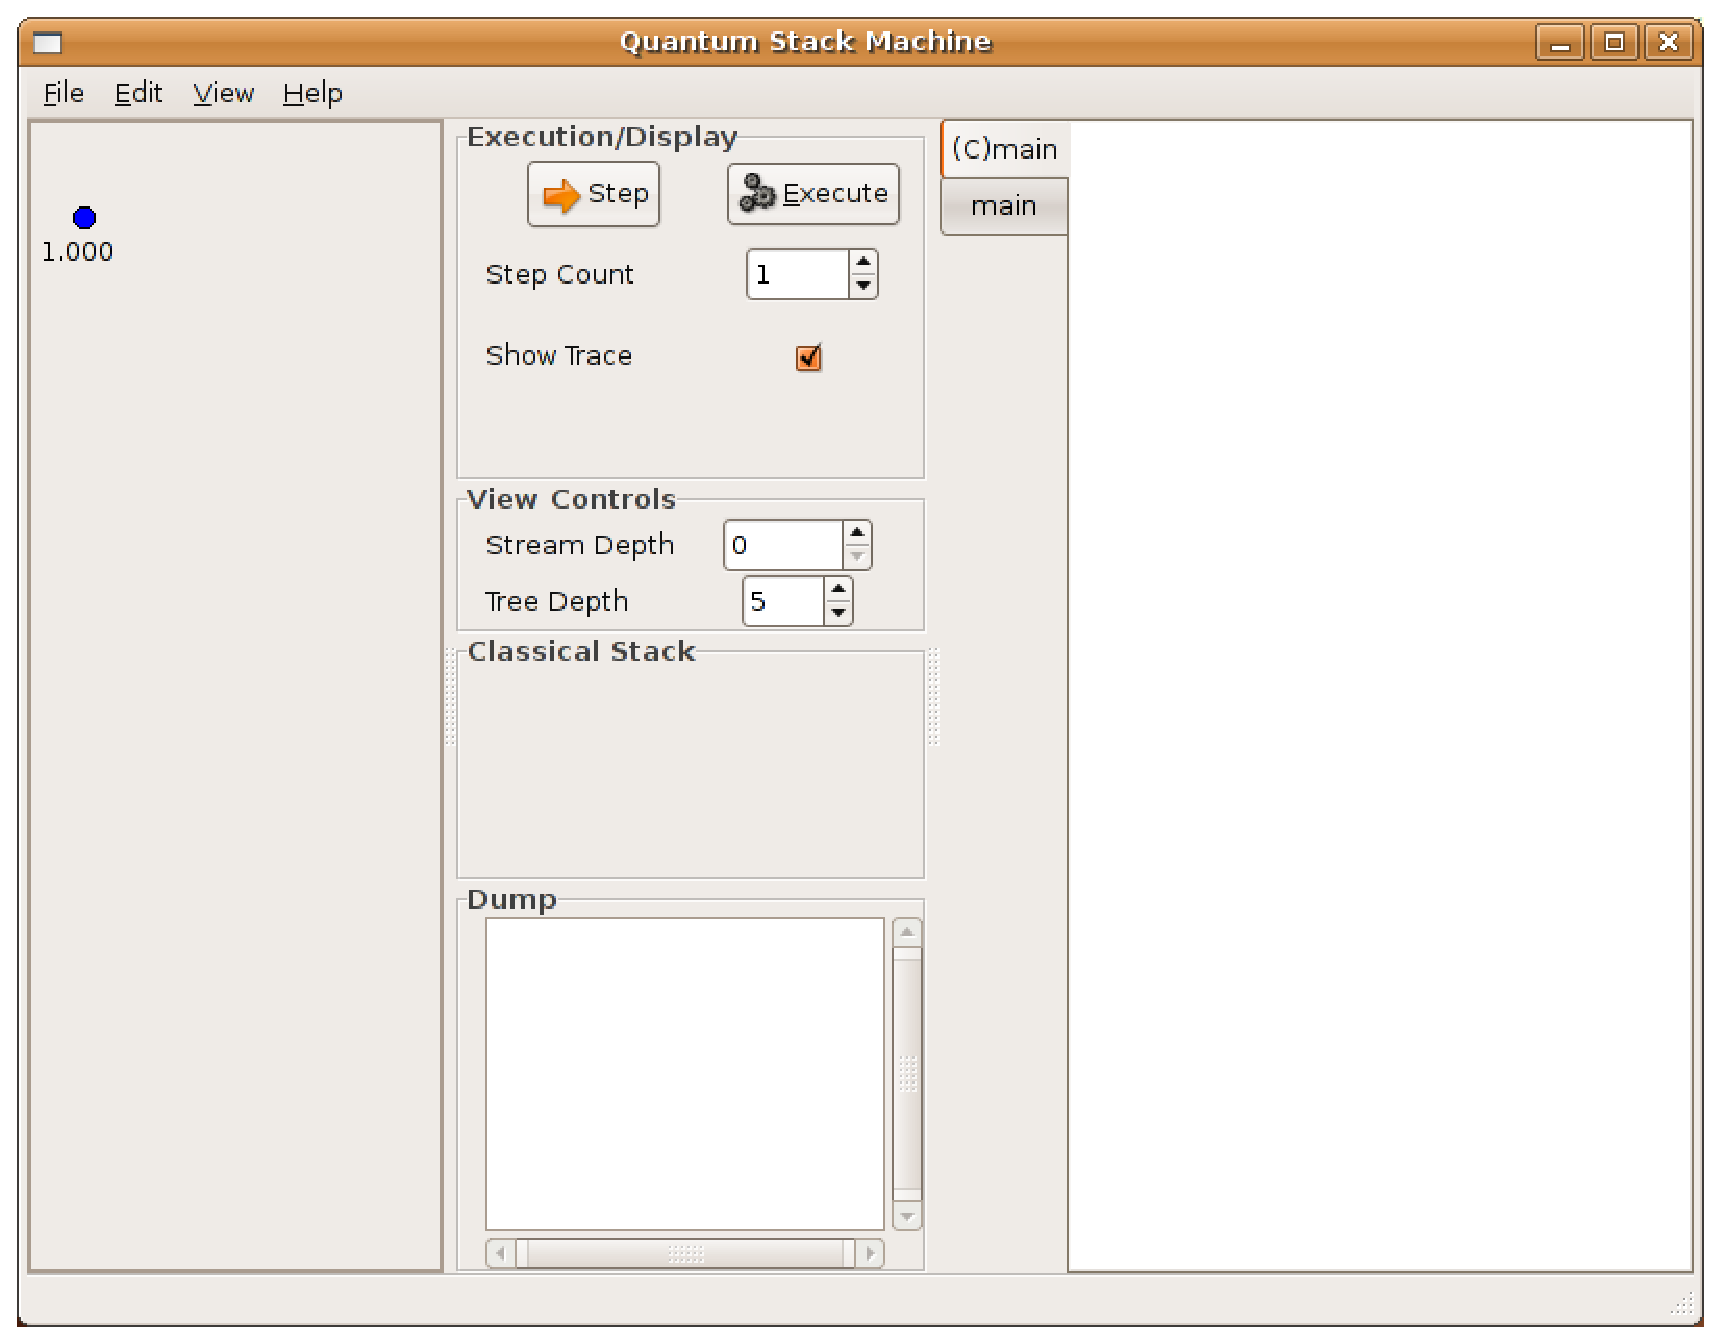
\includegraphics[scale=.5]{images/emulator/EmulatorAtStart.eps}
\caption{The emulator window}\label{fig:emulator}
\end{figure}

The emulator window is composed of three main sections. On the left is
the quantum stack display area. On the right is a tabbed display of the 
emulator assembly/machine code.
 
The middle section is divided into four parts. At the top is 
an execution and display control area followed by a view control area.
Beneath these is the  classical stack display area with
 the dump display area at the bottom.

\subsection{Loading a file}
The first required step is to actually load a program into the emulator,
using the \visctrl{File ---> Open} dialog in \ref{fig:emfileopen}.

\begin{figure}[htbp]
\centering
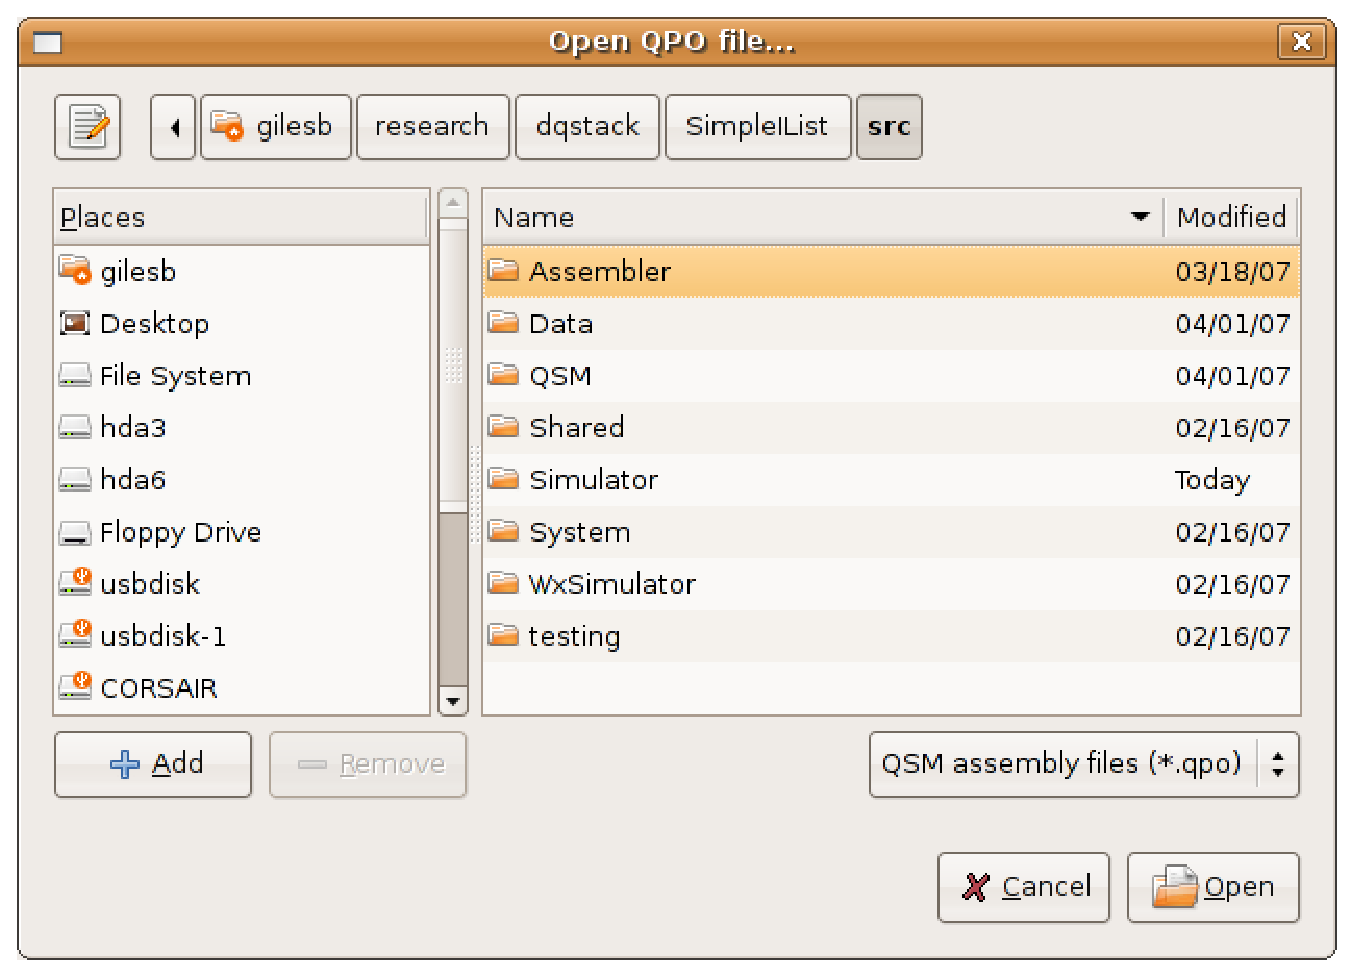
\includegraphics[scale=.5]{images/emulator/OpenDialog.eps}
\caption{Emulator file open dialog}\label{fig:emfileopen}
\end{figure}

Opening a QSM assembly file will check the compiler version 
used to create it and translate it to machine code. If the compiler and
emulator versions do not match, a warning dialog, as 
in \ref{fig:emversionmismatch} will appear. It is suggested that one 
ensures the version of the compiler and emulator are the same. 

\begin{figure}[htbp]
\centering
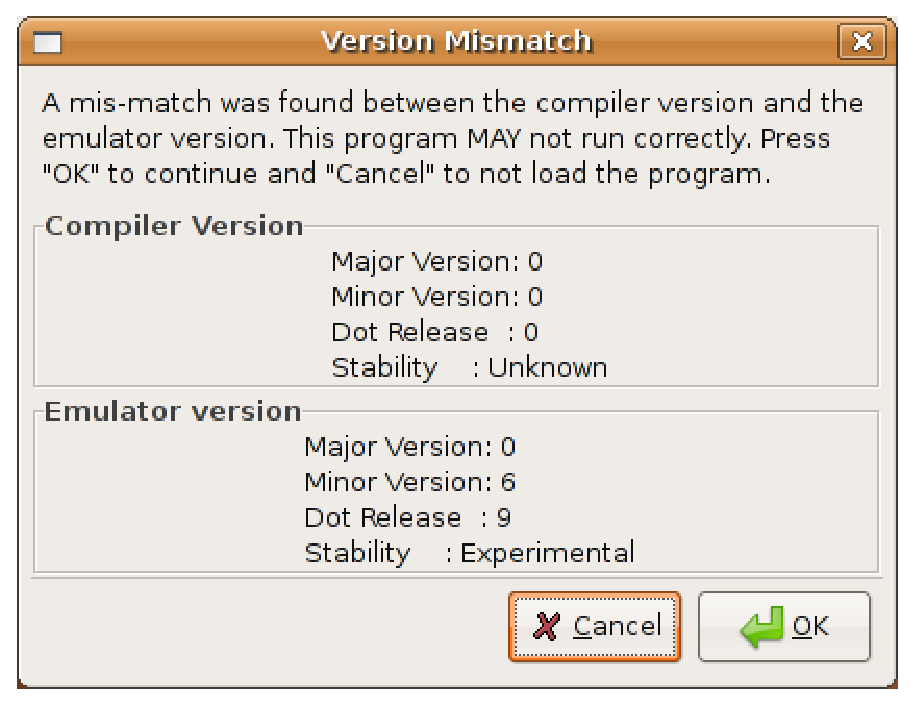
\includegraphics[scale=.5]{images/emulator/VersionMismatch.eps}
\caption{Version mis-match warning}\label{fig:emversionmismatch}
\end{figure}

After a successful assemble, the assembled code will appear in the right 
hand side. In a program, each function will appear as a separate tab in the
tabbed code window. The currently executing code will be in the top tab,
which is labelled with a ``(C)'' and the name of the currently executing 
function. Clicking on a tab will show the code associated with that tab.

\subsection{Setting preferences}

\begin{figure}[htbp]
\centering
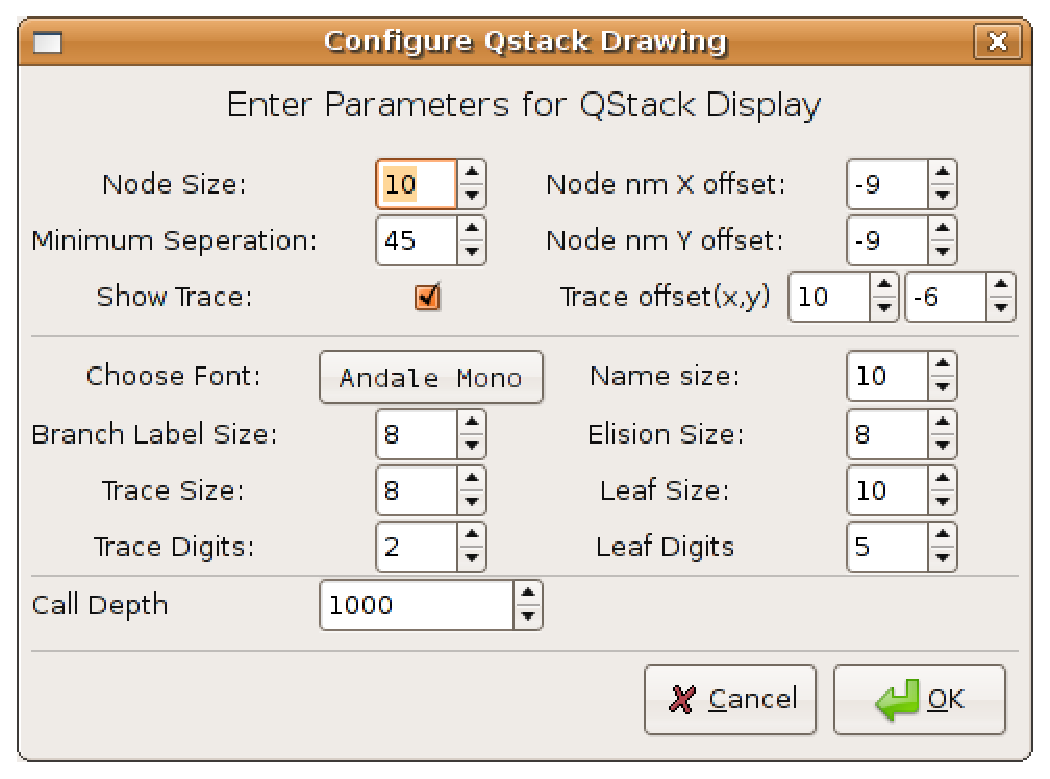
\includegraphics[scale=.5]{images/emulator/ConfigureQstackDisplay.eps}
\caption{Preferences dialog}\label{fig:emconfigure}
\end{figure}

Prior to executing the program, various display and execution options may
be set by using the \visctrl{Edit ---> Preferences} dialog, shown in 
\ref{fig:emconfigure}. The top third of the dialog controls the spacing and
size of nodes and their labels. The middle controls the font used and the 
font size choices for various labels.  Typically, the defaults for these
are sufficient for general execution.  

The final section, with the single item \visctrl{Call Depth} is used
to control the actual depth of recursion \emph{multiplied by the depth in
the stream.} In \ref{fig:emconfigure} the call depth is $1000$, meaning
that at stream depth 0, we will perform 1000 calls before 
signalling non-termination, at stream depth 5, 6000 calls and so on.

\subsection{Running the program}

\begin{figure}[htbp]
\centering
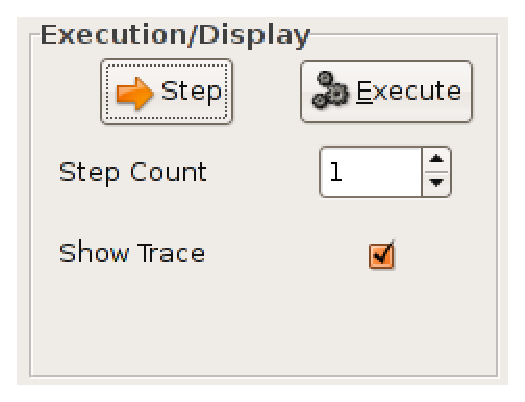
\includegraphics[scale=.8]{images/emulator/ExecutionDisplay.eps}
\caption{Execution control section of the main window}\label{fig:emexecdisplay}
\end{figure}

The program execution is controlled by the elements of the 
\visctrl{Execution/Display} section of the main window. As shown in 
\ref{fig:emexecdisplay}, there are two buttons (\visctrl{Step} and
\visctrl{Execute}), a spin control (\visctrl{Step Count}) and a 
checkbox (\visctrl{Show Trace}).

For each click of the \visctrl{Step} button, the emulator will execute
\emph{\visctrl{Step Count}} instructions and then redisplay the 
components of the quantum stack machine. The spin control may be set to 
any positive number.

The \visctrl{Execute} button will run the program until it completes. 
Completion may either be due to non-termination (e.g., exceeding the call
depth number of calls at the current stream depth), or actual completion.
See the  description of \visctrl{Stream Depth} below.
As well, while executing, the program will display a progress bar below the
\visctrl{Show Trace} area.  After completion, the machine components will
be re-displayed.

\begin{figure}[htbp]
\centering
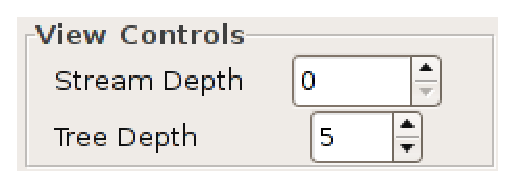
\includegraphics[scale=.8]{images/emulator/ViewControls.eps}
\caption{View controls section of the main window}\label{fig:emviewcontrols}
\end{figure}

The other component that affects execution in both  step mode and 
execute mode is the \visctrl{Stream Depth}, shown 
in \ref{fig:emviewcontrols}. Essentially, if one encounters a 
non-termination (a zero quantum stack) after executing, just increase the 
\visctrl{Stream Depth} and continue.

\subsection{Result interpretation}
Obviously, the first step is to visually examine the quantum stack. In case
where a simple final result is produced, this is often enough.

However, in cases where there are a significant number of nodes with multiple
branches, it can be difficult to determine what the results actually are.

\begin{figure}[htbp]
\centering
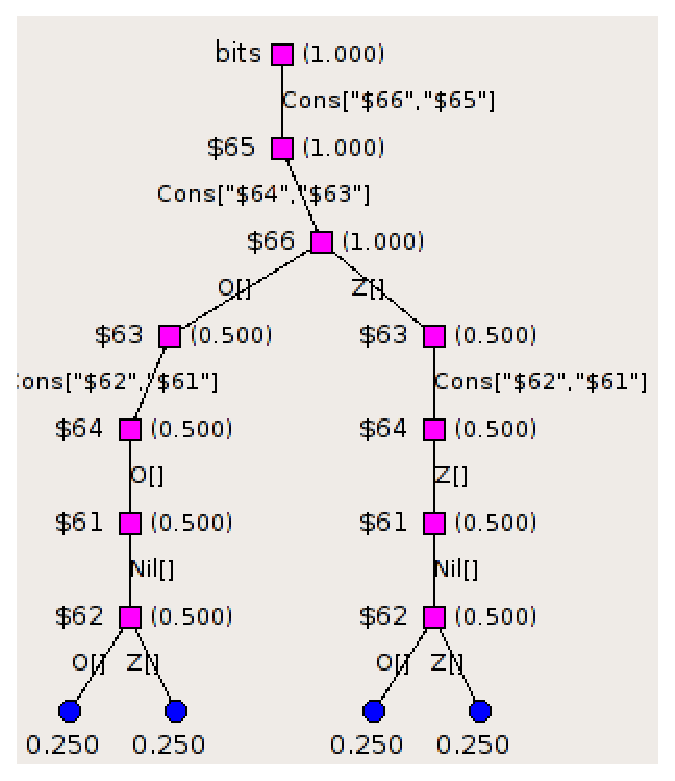
\includegraphics[scale=.75]{images/emulator/SimonsResult.eps}
\caption{Quantum stack at end of Simon's algorithm}\label{fig:emsimonsresult}
\end{figure}

For example, consider the end result of running Simon's algorithm, as shown
in \ref{fig:emsimonsresult}. The important result is ``What are the 
resulting bit-strings?''\footnote{Obviously, it is possible to determine 
the results solely by examination of the quantum stack as displayed. The 
method shown here becomes more relevant the more complicated the 
result stack.}. Using the menu item \visctrl{File ---> Simulate}, we
bring up a simulation dialog, which does the ``roll the dice'' and 
shows us what our end result would be when transferred to a classical
computer. For example, for three invocation of simulation, we 
get sub-figures (a), (b), and (c) as shown in \ref{fig:emsimonsims}.

\begin{figure}[htbp]
\centering
\subfloat[First simulation]{
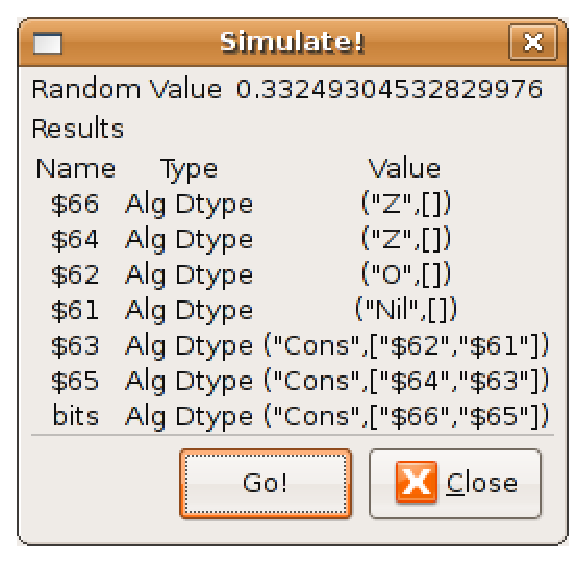
\includegraphics[scale=.7]{images/emulator/SimonsSimulate1.eps}
}
\subfloat[Second simulation]{
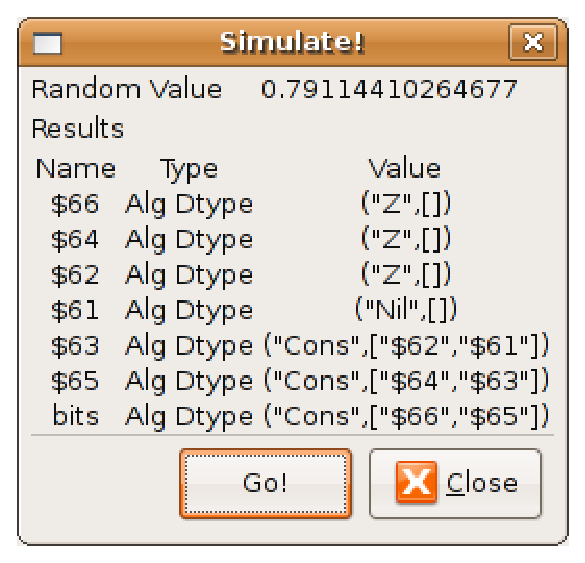
\includegraphics[scale=.7]{images/emulator/SimonsSimulate2.eps}
}
\subfloat[Third simulation]{
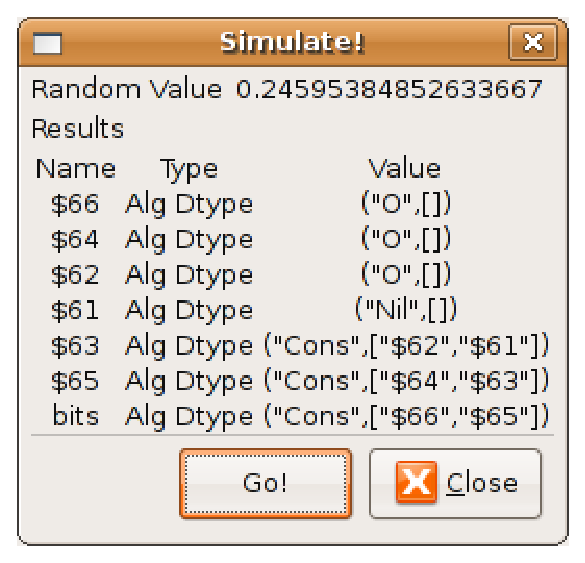
\includegraphics[scale=.7]{images/emulator/SimonsSimulate3.eps}
}
\caption{Simulation of  Simon's algorithm}\label{fig:emsimonsims}
\end{figure}

Note that the bit string can simply be read from the top three entries 
in the simulation results. It should also be noted that the additional
simulations do not require re-execution by the emulator. Instead, a new
random value is generated and used to determine a single path down the 
quantum stack for the values.





\bibliographystyle{amsalpha}
\bibliography{lqplbib}
\labelformat{chapter}{appendix~#1}
\labelformat{section}{appendix~#1}
\labelformat{subsection}{appendix~#1}
\labelformat{subsubsection}{appendix~#1}
\appendix
\chapter{The quantum stack machine}\label{chap:quantumStackMachine}
\section{Introduction to the quantum stack machine}\label{sec:introStackMachine}
The quantum stack machine provides an execution environment where
 quantum and classical data may be manipulated. The primary component
of this machine is the \emph{quantum stack}, which stores both quantum and
probabilistic data.

The quantum stack  has the same function as a  classical stack 
in that it provides the basic
operations and data structures
 required for quantum computation. 

For the semantics of this, please refer to \cite{giles:msc2}.

This chapter  describes a machine using this full quantum stack and other
data structures to provide an execution environment for \lqpl{} programs.


\section{Quantum stack machine in stages}\label{sec:qsmstate}
The quantum stack machine is described in terms of four 
progressively more elaborate stages. The first stage is
the   \emph{basic QS-machine}, labelled \bms. This stage provides
 facilities for the majority of operations
of our machine, including classical operations, adding and discarding data
 and classical control. The second stage, the \emph{labelled QS-machine},
called \lbms{} adds the capability of applying 
unitary transforms with the modifiers 
\semins{Left, Right} and \semins{IdOnly} as introduced in 
\cite{giles:msc2}. 
The third stage, the  \emph{controlled QS-machine}, is labelled \cms{} and 
provides the
ability to do quantum control. The final stage,  the
\emph{QS-machine}, is labelled \ms{} and 
 adds the ability to call subroutines and do 
recursion.

These stages are ordered in terms of complexity and the
operations definable on them. The ordering is:
\[ \bms < \lbms < \cms < \ms\]
When a function is defined on one of the lower stages, it is possible
to lift it to a function on any of the higher stages. 

%The details of the Haskell implementation of 
%these stages and the lifting functions are given in 
%\vref{subsec:QSM:machinedescription}.

\subsection{Basic quantum stack machine}\label{subsec:basicmachinestate}

The quantum stack machine transitions for the quantum instructions 
 are defined  at this stage.
The state of the basic quantum stack machine  has a code stream, $\cd$, a
classical stack, $S$, a  quantum stack, $Q$, a dump, $D$ and a
name supply, $N$.
\begin{equation}
(\cd,S,Q,D,N)\label{eq:minimalmachinestate} \\
\end{equation}

The code, $\cd$,  is a list of machine instructions. Transitions 
effected by these instructions are detailed in 
 \vref{subsec:transitiondiagrams}. English descriptions of the
instructions and what they do are given in 
 \vref{subsec:repauxinstructions}.


The classical stack, $S$, is a standard stack whose items may
be pushed or pulled onto the top of the stack and specific locations 
may be accessed for both reading and updating.
Classical arithmetic and Boolean operations are done with the top
elements of the classical stack. Thus, an add will pop the
top two elements of the classical stack and then push the result 
 on to the top of the stack.


The dump, $D$, is a holding area for intermediate results and returns. This
is used when measuring quantum bits,  using probabilistic data, 
splitting constructed data types and for calling subroutines. Further
details are given in \vref{sec:representationofdump}.


The name supply, $N$, is an integer that is incremented each
time it is used. The name supply is used when binding nodes to 
constructed data nodes. As they are bound, they are renamed to a unique name
generated from the name supply. For further details on this, see 
the transitions for \qsmins{QBind} at \vref{subsec:quantumstacknodecreation}.

\subsection{Labelled quantum stack machine}\label{subsec:labelledmachinestate}

The labelled QS-machine, designated as \lbms, extends  \bms{} by
labelling the quantum stack, $L(Q)$. The quantum stack is labelled to 
control the application of
 unitary transformations, which allows quantum control to
be implemented.

The labelled QS-machines state is a tuple of five elements:
\begin{equation}
(\cd,S,L(Q),D,N)\label{eq:minimalmachinestateplus}
\end{equation}

The quantum stack is labelled by one of four labels: 
\texttt{Full, Right, Left} or 
\texttt{IdOnly}. These labels 
describe how unitary transformations will be applied to  the quantum stack.

When this labelling was introduced in \cite{giles:msc2}, it 
was used as an instruction modifier rather than a labelling of the
quantum stack. While the implementation of these modifiers  is
changed, the effect on the quantum stack is the same. The quantum stack
machine transitions for unitary transformations are detailed 
in  \vref{subsec:trans:unitarytransformations}.


\subsection{Controlled quantum stack machine}\label{subsec:controlledmachinestate}

The controlled quantum stack machine, \cms, adds the capability to 
 add or remove quantum control.
This stage  adds a control stack, $C$, and changes the 
 tuple of classical stack, labelled quantum stack, dump
and name supply into a  list of tuples of these elements. In the 
machine states, a list will be denoted by enclosing the list items
or types in square brackets.

The \cms{} state is a tuple of three elements, where the third element
is a list of four-tuples:
\begin{equation}
(\cd, C , [(S,L(Q),D,N)]) \label{eq:controlmachinestate}
\end{equation}



The control stack is implemented using 
a list of functions, each of which is defined on the third element of
\cms. The functions in the control stack
transform the list of  tuples $(S,L(Q),D,N)$.  Control points are
added to the control stack 
by placing an identity function at the top of
the stack. Control points are removed by taking the top of the control stack
and applying it to the current third element of \cms, resulting in
a new list of tuples.
Adding a \qubit{} to control will modify the function on top of the control
stack
and change the list of tuples of $(S,L(Q),D,N)$.

\subsection{The complete quantum stack machine}\label{subsec:machinestate}

The complete machine, \ms,  allows the  implementation of  subroutine calling.
Its state consists of 
an infinite list of \cms{} elements.

\begin{equation}
\Inflist{(\cd, C , [(S,L(Q),D,N)])} \label{eq:machinestate}
\end{equation}


Subroutine calling is done in an iterative manner. At the head of the
infinite list, no subroutines are called, but result in divergence.
Divergence is represented in the quantum stack machine by a quantum 
stack with a trace of $0$.

In the next position of the infinite list, a subroutine will be entered once.
If the subroutine
 is recursive or calls other subroutines, those calls will diverge. 
The next position of the infinite list will call one more
level. At the $n^{\mathrm{th}}$ position of the infinite list 
subroutines are executed to a call depth of $n$.

\subsection{The classical stack}\label{subsec:repauxclassicalstack}
The machine uses and creates values
on the classical stack when performing arithmetic operations. 
This object is a standard 
push-down stack with random access.
Currently it accommodates both integer and Boolean values.

\subsection{Representation of the dump}\label{sec:representationofdump}
When processing various operations in the machine, such as  those
labelled as quantum control (measure et. al.), the machine will 
need to save intermediate stack states and results. To illustrate, when 
processing a case deconstruction of a datatype,
the machine saves all partial trees of the node on the dump together
with an empty stack to accumulate
 the results of processing these partial trees.
After processing  each case the current quantum stack is
merged with the result stack and the next partial stack is processed. 
The classical stack is also saved in the
dump element at
the beginning of the process and reset to this saved value 
when each case is evaluated.


The dump is  a list of \emph{dump elements}. There are two distinct types
of dump elements, one for quantum control instructions and one used for
  call statements. The details of these elements may
be found in the description of the quantum control transitions in
 \vref{subsec:measurementandchoice} and 
function calling in \vref{subsec:functioncalling}.

\subsection{Name supply}
The name supply is a read-only register of the machine. It 
provides a unique name
when binding nodes to a data node. The implementation 
uses an integer value which
is incremented for each of the variables in a selection pattern in
a case statement. It is reset to zero at
the start of each program.

%\input{secTransformStates} Note about transforming added to Intro.
\section{Representation of data in the quantum stack}\label{subsec:representationofqstackdata}

The quantum stack was introduced and described in \cite{giles:msc2} in the chapeter on semantics.
 This
section will give further details of the implementation of the quantum
stacks and show example nodes.

\subsection{Representation of \qubit{}s.}\label{subsec:representationOfQubits}
A single \qubit{} is represented on the quantum stack as a  node with
four possible branches. This assumes a basis for quantum computation
of two elements, which is identified with $(0,1)$ and $(1,0)$ in 
 $\complex^2$. The four possible values of the branches represent
the elements of the \qubit{}'s density matrix. This is illustrated in
\vref{fig:lqplHadQubit}. From left to right, the branches are labelled with
$00, 01, 10$ and $11$. The value at each branch is $.5$. This 
corresponds to the density matrix {\begin{singlespace}
$\begin{bmatrix}.5&.5\\.5&.5\end{bmatrix}$\end{singlespace}
}

\begin{figure}[htbp]
\centerline{
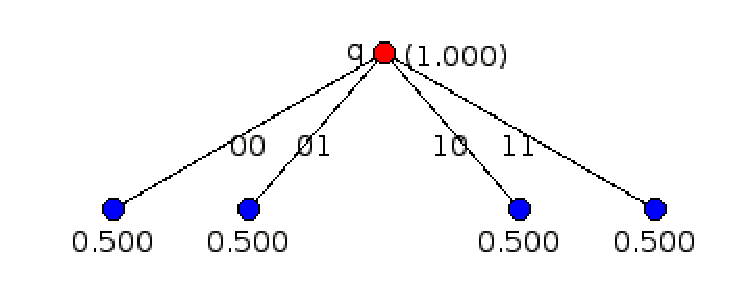
\includegraphics[scale=.6]{images/HadQubit.eps}
}
\caption{A \qubit{} after a \Had{} transform}\label{fig:lqplHadQubit}
\end{figure}

With multiple \qubit{}s,  the representation becomes hierarchical.
For example, two \qubit{s} will be represented by a tree with one of the
\qubits{} at the top and each of its sub-branches
 having the second \qubit{} below it. 
Consider applying a Hadamard transform to one \qubit, followed by a 
controlled-Not with that \qubit{} as the control. This is 
a standard way to entangle two \qubits. As illustrated in
\vref{fig:entangled}, this creates a tree in the quantum stack with
a total of four non-zero leaves. The quantum stack in the figure
corresponds to a sparse representation of the density matrix:

{\begin{singlespace}
\[\left[
\begin{array}{c|c}
\begin{array}{cc}
.5&0\\0&0
\end{array} &
\begin{array}{cc}
0&.5\\0&0
\end{array}\\
\hline
\begin{array}{cc}
0&0\\.5&0\\
\end{array} &
\begin{array}{cc}
0&0\\0&.5
\end{array}
\end{array}\right]
\]
\end{singlespace}
}

\begin{figure}[htbp]
\centerline{
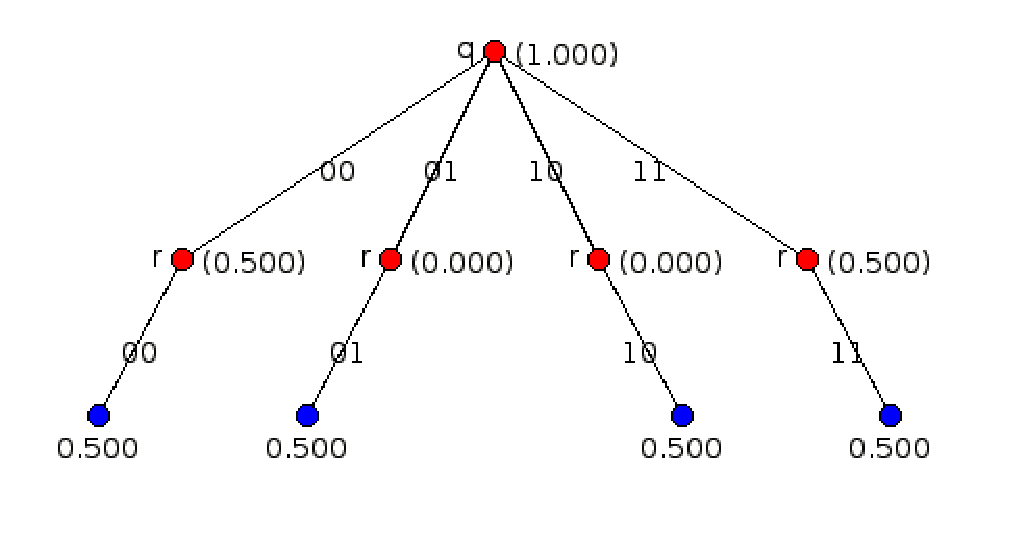
\includegraphics[scale=0.6]{images/entangledQubits.eps}
}
\caption{Two entangled \qubits}\label{fig:entangled}
\end{figure}

\subsection{Representation of integers and Boolean values}\label{subsec:representclassicaldata}
Numeric and Boolean
 data in the quantum stack machine is represented by a node with
a sub-branch for each value that occurs with a non-zero probability. 
These values may be of either integer or Boolean type.

\begin{figure}[htbp]
\centerline{
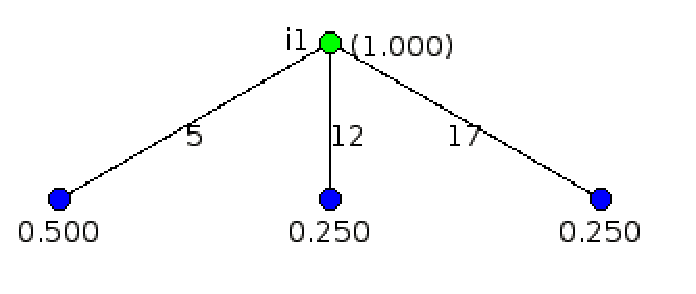
\includegraphics[scale=.6]{images/integer.eps}
}
\caption{An integer with three distinct values}\label{fig:integerofthree}
\end{figure}

\Vref{fig:integerofthree} depicts an
integer $i1$ which has 
a $50\%$ probability of being $5$, and $25\%$ each of being $12$ or $17$.

\subsection{Representation of general data types}\label{subsec:representgeneraldatatyps}
The general datatype is represented 
as a node with one branch for each of the constructors that occurs
with a non-zero probability. Each branch is labelled by the 
constructor and the names of any nodes that are 
bound to it\footnote{For example, in \qtype{List}s of 
integers, the
\qcons{Cons} constructor requires a base integer and another \qtype{List}.}.
These
nodes will be referred to as  \emph{bound nodes}.


\begin{figure}[htbp]
\centerline{
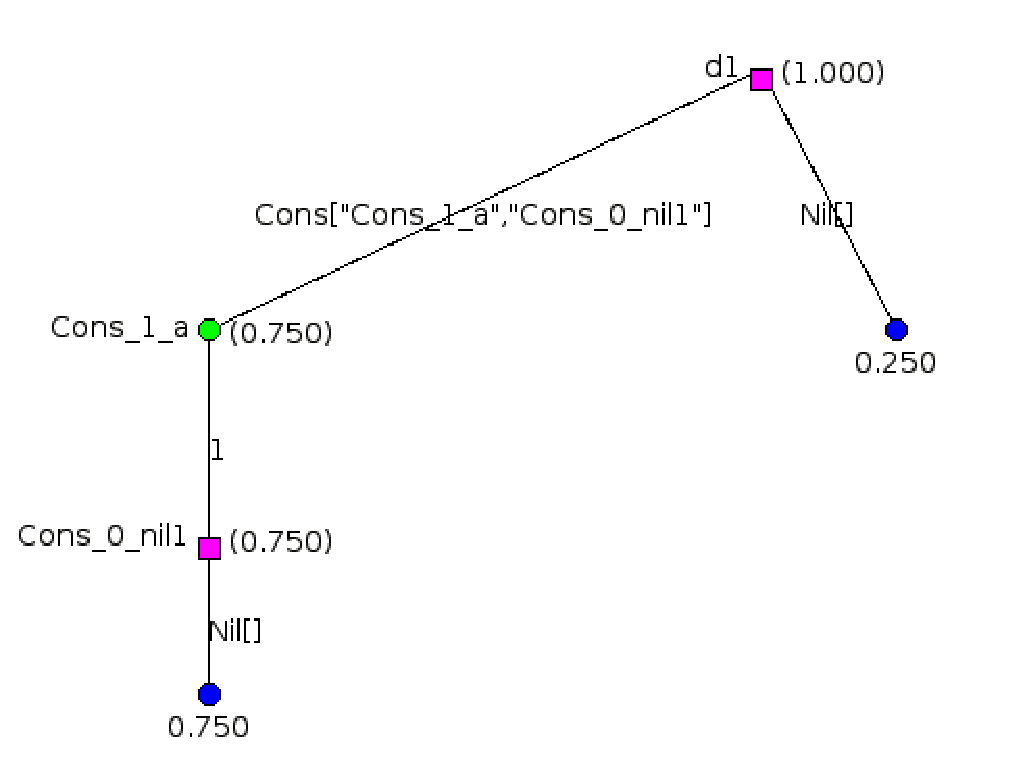
\includegraphics[scale=.75]{images/listExample.eps}
}
\caption{A list which is a mix of $[\ ]$ and $[1]$.}\label{fig:schizolist}
\end{figure}



For example, in the \qtype{List} that appears in \vref{fig:schizolist}, 
the top node  is a mix of values. The node $d1$ has a $25\%$ chance of 
being \qcons{Nil} and $75\%$ of being a \qcons{Cons} of two bound nodes.
The first bound node is an element of the base type, integer. 
It is labelled \terminalio{Cons\_1\_a} which
is an integer node having the single value 1. The second bound element is 
\terminalio{Cons\_0\_nil1},  which is another list having the
 single value of \qcons{Nil}. 





\section{Quantum stack machine operation}\label{sec:stackmachineoperation}
This section describes the actual transitions of the stack
machine for each of the instructions in the machine.

\subsection{Machine transitions}\label{subsec:transitiondiagrams}
The majority of the transitions presented in this section are 
defined on 
a machine of type $\bms = (\cd,S,Q,D,N)$ as was 
introduced in \vref{subsec:basicmachinestate}.
As discussed in that section, labelling only affects the
transition of unitary transforms. All other instruction transitions 
ignore it, giving us:
\[ Ins(L(Q)) = L (Ins (Q)) \]
where $Ins$ is the transition of some other instruction.

The transition for the application of transformations will use \lbms, while
the transition for the add/remove control instructions 
uses the machine state of  \cms. 
The call instruction uses the 
state of the complete machine, \ms, which allows recursion.
All of these stages and their associated states were defined and discussed 
in  \vref{sec:qsmstate}.



\subsection{Node creation}\label{subsec:quantumstacknodecreation}
There are three instructions which allow us to create data on the 
stack and one which binds sub-nodes into a data type. These are 
\qsmins{QLoad, QCons, QMove} and \qsmins{QBind}. The transitions are shown
in \vref{fig:trans:nodeconstruction}.

The instructions do the following tasks:
\begin{description}
\item{\qsminswithp{QLoad}{nm\ \ket{i}}} --- Load a new \qubit{} named 
\qsminsparm{nm} on top of the quantum stack with the value \ket{i};
\item{\qsminswithp{QCons}{nm\ Cns}} -- Load a new datatype node on top of the
quantum stack with name \qsminsparm{nm} and value \qsminsparm{Cns}.
Sub-nodes are not bound  by this instruction.
\item{\qsminswithp{QMove}{nm}} --- Load a new classical node on top of the
quantum stack with name \qsminsparm{nm} and value taken from the
top of the classical stack. If the classical stack is empty, the
value is defaulted to $0$.
\item{\qsminswithp{QBind}{nm}} --- Binds a sub-node down the 
branch of the node to the datatype constructor on top of the 
quantum stack. Furthermore, the act of binding will
cause the newly bound sub-node to be renamed so that it is
hidden until an unbind is performed. \qsmins{QBind} 
uses the name supply,
$N$, to create the new  name for the sub-node. The machine will
generate an exception if the top of the quantum stack is not a
single branched datatype or if a node named \qsminsparm{nm} is not found. 
\end{description}


\begin{figure}[htbp]
\begin{tabular}{l}
$(\mathrm{QLoad}\ x\ \ket{k}{:}\cd,S,Q,D,N)  $ \\
$ \trspace\implies(\cd,S,x{:}[\ket{k}\to Q],D,N)$ \\
$(\mathrm{QCons}\ x\ c{:}\cd,S,Q,D,N) $ \\
$ \trspace\implies (\cd, S,x{:}[c\{\}\to Q],D,N) $ \\
$ (\mathrm{QMove}\ x{:}\cd,v{:}S,Q,D,N) $ \\
$ \trspace\implies (\cd,S,x{:}[\bar{v}\to Q],D,N)$ \\
$(\mathrm{QBind}\ z_0{:}\cd,S,x{:}[c\{z_1',\ldots,z_n'\}\to Q],D,N) $\\
$ \trspace \implies (\cd,S,x{:}[c\{z(N),z_1',\ldots,z_n'\}\to Q[z(N)/z_0]],D,N') $
\end{tabular}
\caption{Transitions for node construction}\label{fig:trans:nodeconstruction}
\end{figure}



\subsection{Node deletion}\label{subsec:nodedeletion}

Three different instructions, \qsmins{QDelete, QUnbind} and \qsmins{QDiscard}
 remove data from the 
quantum stack.  These instructions are the converses of \qsmins{QBind}, 
\qsmins{QLoad} and \qsmins{QMove}. Their transitions are shown in
\ref{fig:trans:nodedestruction} and \ref{fig:trans:noderemoval}.
The instructions do the following tasks:
\begin{description}
\item{\qsmins{QDelete}} --- removes the top node of the stack 
\emph{and any bound sub-nodes}. This instruction has no restrictions on
the number of sub-stacks or bindings in a data node;
\item{\qsmins{QDiscard}} --- removes the top node of the stack. In all cases,
the top node can only be removed when it has
a single sub-stack. For datatype nodes, \qsmins{QDiscard} also requires
there are no bound sub-nodes.
\item{\qsminswithp{QUnbind}{nm}} --- removes the
 first bound element from a data type 
\emph{provided it has a single sub branch}. The datatype node must be
 on top of the quantum stack. The newly unbound sub-node is renamed
 to \qsminsparm{nm}.
\end{description}


\begin{figure}[htbp]
\begin{tabular}{lll}
$(\mathrm{QDelete}{:}\cd,S,Q{:}[\ket{k_{ij}}\to Q_{ij}],D,N)$&$ \implies $&$(\cd,S,(Q_{00}+Q_{11}),D,N)$ \\[12pt]
$(\mathrm{QDelete}{:}\cd,S,DT{:}[c_i\{b_{ij}\} \to Q_i],D,N)$&$ \implies $&$(\cd,S,\sum_i(del(\{b_{ij}\}, Q_i)),D,N)$ \\[12pt]
$(\mathrm{QDelete}{:}\cd,S,I{:}[\overline{v}_i \to Q_i],D,N)$&$ \implies $&$(\cd,S,\sum_i Q_i,D,N)$ 
\end{tabular}
\caption{Transitions for destruction}\label{fig:trans:nodedestruction}
\end{figure}

For the \qsmins{QDelete} instruction, the type of node is irrelevant.
It will delete the node and, in the case of datatype nodes, any
bound nodes. This instruction is required to implement 
sub-routines that have parametrized datatypes as input arguments.
For example, the algorithm for determining the length of a
list is to return $0$ for the ``Nil'' constructor and 
add $1$ to the length of the tail list in the ``Cons'' constructor. 
When doing this, the elements of the list are deleted due to the 
linearity of \lqpl.
The compiler will have no way of determining the type of the 
elements in the list and
therefore could not generate the appropriate quantum split and discards.
The solution is to use a \qsmins{QDelete} instead.

The subroutine $del$ used in the transitions 
in \ref{fig:trans:nodedestruction}
will recursively rotate up and then delete the bound nodes of a datatype
 node.


\begin{figure}[htbp]
\begin{tabular}{lll}
$(\mathrm{QDiscard}{:}\cd,S,x{:}[\ket{k}\to Q],D,N) $&$ \implies$&$ (\cd,S,Q,D,N)$ \\[12pt]
$(\mathrm{QDiscard}{:}\cd,S,x{:}[c\{\} \to Q],D,N) $&$\implies $&$(\cd,S,Q,D,N)$ \\[12pt]
$(\mathrm{QDiscard}{:}\cd,S,x{:}[\overline{v} \to Q],D,N) $&$\implies$&$ (\cd,v{:}S,Q,D,N)$ \\[12pt]
\multicolumn{3}{l}{$(\mathrm{QUnbind}\ y{:}\cd,S,x{:}[c\{z_1',\ldots,z_n'\}\to Q],D,N) $} \\
\multicolumn{3}{r}{$\trspacefour\trspacethree\quad\ \ \implies\ \ \ (\cd,S,x{:}[c\{z_2',\ldots,z_n'\} \to Q[y/z_1']],D,N)$}
\end{tabular}
\caption{Transitions for removal and unbinding}\label{fig:trans:noderemoval}
\end{figure}



 The 
renaming is an integral part of the \qsmins{QUnbind}
instruction, as a compiler will not be able to know  the bound names of
a particular data type node. The instruction 
does \emph{not} delete the data type at the top of the stack or
the unbound node. If the top node is not a data type or has more than
a single branch or does not 
have any bound nodes, the machine will generate an exception. 

The machine ensures that it does not create  name capture issues
by rotating the bound node to the top of the sub-stack before
it does the rename. That is, given the situation as depicted in
the transitions, the quantum stack machine performs the 
following operations:

{\begin{singlespace}
\begin{enumerate}
\item{} $ Q' \leftarrow pull(z_1',Q)$;
\item{} $ Q'' \leftarrow  Q'[y/z_1'] $;
\item{} $z_1'$ is removed from the list of constructors;
\item{} The new quantum stack is now set to $x{:}[c\{z_2',\ldots,z_n'\} \to Q'']$.
\end{enumerate}
\end{singlespace}
}



\subsection{Stack manipulation}\label{subsec:stackmanipulation}
Most operations on a quantum stack affect only the top of the stack.
 Therefore,  the machine must have
 ways to move items up the stack. This requirement is met by the instructions
\qsmins{QPullup} and \qsmins{QName}. The transitions are shown in 
\vref{fig:trans:manipulation}.

The instructions do the following tasks:
\begin{description}
\item{\qsminswithp{QPullup}{nm}} --- brings the \emph{first} node named 
\qsminsparm{nm} to the top of the quantum stack. 
It is not an error to try pulling up a non-existent address. The original
stack will not be changed in that case.
\item{\qsminswithp{QName}{nm_1\ nm_2}} --- renames the first
node in the stack having \qsminsparm{nm_1} 
to \qsminsparm{nm_2}.
\end{description}

\begin{figure}[htbp]
\begin{tabular}{lll}
$(\mathrm{QPullup}\ x{:}\cd,S,Q,D,N) $&$\implies$&$ (\cd,S,\mathrm{\textsf{pull}}(x,Q),D,N)$ \\[12pt]
$(\mathrm{QName}\ x\ y{:}\cd,S,Q,D,N) $&$\implies$&$ (\cd,S,Q[y/x],D,N)$ 
\end{tabular}
\caption{Transitions for quantum stack manipulation}\label{fig:trans:manipulation}
\end{figure}

A \qsminswithp{QPullup}{nm} has the potential to be
an expensive operation as the node \qsminsparm{nm} may be 
deep in the quantum stack . In practice, many
 pullups interact  with only the top two or three elements of the
quantum stack.

The algorithm for pullup is based on preserving the bag of 
\emph{path signatures}.  A {path signature} for a node
consists of a bag of ordered pairs (consisting of the node name and
the branch constructor) where
every node from the top to the leaf is represented. 
Pulling up a
node will reorder the sub-branches below nodes to keep this invariant.

Due to the way  arguments of recursive subroutines are handled in \lqpl,
it is actually possible to get multiple nodes with the same name, however, this
does not cause a referencing problem as only the highest such node is actually
available in the \lqpl{} program.

\subsection{Measurement and choice}\label{subsec:measurementandchoice}
The instructions
\qsmins{Split}, \qsmins{Measure} and \qsmins{Use} start the task of 
operating on a node's partial stacks, while the fourth, \qsmins{SwapD} 
is used to iterate through the partial stacks. The transitions are shown in 
\vref{fig:trans:measures}.

The instructions do the following tasks:
\begin{description}
\item{\qsminswithp{Use}{(Lbl,EndLbl)}} --- uses the classical node at the top
of the quantum stack and executes the code at \qsminsparm{Lbl} for
each of its values. When done, jump to \qsminsparm{EndLbl}.
\item{\qsminswithp{Split}{([(c_1,lbl_1),\dots,(c_n,lbl_n)],EndLbl)}} --- uses the
datatype node at the top of the stack and
execute a jump to the code 
at \qsminsparm{lbl_i} when there is a branch having constructor
\qsminsparm{c_i}. Any constructors not mentioned in the instruction 
are removed from the node first. There is no ordering 
requirement on the pairs of constructors and labels in \qsmins{Split}. When all 
pairs have been processed, jump to \qsminsparm{EndLbl}.
\item{\qsminswithp{Measure}{(Lbl_{00},Lbl_{11},EndLbl)}} --- using the
\qubit{} node on top of the quantum stack, executes
 the code at the first two labels for 
 the \qsminsparm{00} and \qsminsparm{11} branches. 
The off-diagonal elements  of the \qubit{} will be
discarded. This implements a 
non-destructive measure of the \qubit. When done, jump to \qsminsparm{EndLbl}.
\item{\qsmins{SwapD}} --- signals the end of processing of dependent 
instructions and begins processing the next partial stack.
 When all values are processed, merges the results and returns
to the instruction labled by \qsminsparm{EndLbl} from the corresponding \qsmins{Measure}, \qsmins{Use}
or \qsmins{Split} instruction.
\end{description}
Note that in all cases above, these instructions execute a jump and the code following the 
instruction is not used per se. Naturally, the code following may be addressed by a label and therefore
will be executed. The \texttt{lqpl} compiler normally generates the code from one of these in
this layout:
\begin{verbatim}
      Enscope
      Split @c lbl3 (#Cons1,lbl1) (#Cons2, lbl2)
lbl1  Discard @c
      ...
      SwapD
lbl2  Discard @c
      ...
      SwapD
lbl3  Descope
      ...
\end{verbatim}
\begin{figure}[htbp]
\begin{tabular}{l}
$(\mathrm{Use}\ (\lbl_U,\lbl_{E}){:}\_,S,x{:}[\bar{v_i}\to Q_i],D,N) $ \\
$\trspacetwo\implies (\cd_U,S,x_1{:}v_1\to Q_1, 
	\dmpelemqc{}(S,[(x_i{:}v_i\to Q_i,\lbl_U)]_{i=2,\ldots,n},\lbl_E, 0){:}D,N)$ \\[12pt]
$(\mathrm{Split}\ ([(c_i,\lbl_i)],\lbl_E){:}\_,S,x{:}[c_i\{V_i\}\to Q_i],D,N) $ \\
$\trspacetwo\implies (\cd_1,S,x_1{:}c_1\{V_1\}\to Q_1, 
	\dmpelemqc{}(S,[(x_i{:}c_i\{V_i\}\to Q_i, \lbl_i)]_{i=2,\ldots,n},\lbl_E, 0){:}D,N)$ \\[12pt]
$(\mathrm{Meas}\ (\lbl_0, \lbl_1,\lbl_E){:}\_,S,x{:}[\ket{0}\to Q_0,\ket{1}\to Q_1],D,N) $ \\
$\trspacetwo\implies (\cd_0,S,(x_0{:}\ket{0}\to Q_0, 
       \dmpelemqc{}(S,[(x_1{:}\ket{1}\to 
	Q_1,\lbl_1)],\lbl_E, 0){:}D,N)$ \\[12pt]
\\
$(\mathrm{SwapD},S',Q,\dmpelemqc{}(S,
	[(Q_i,\lbl_i)]_{i=j,\ldots,m},\cdptr, Q'){:}D,N) 
       $ \\
$\trspacetwo\implies (\lblcd_j,S,Q_j, \dmpelemqc{}
	(S,[(Q_i,\lbl_i)]_{i=j+1,\ldots,m},\cdptr,Q+Q'){:}D,N)$ \\[12pt]
$(\mathrm{SwapD},S',Q,\dmpelemqc{}(S,[],\cdptr, Q'){:}D,N) 
       $ \\
$\trspacetwo\implies (\cd,S,Q+Q', D,N)$\\[12pt]
Specifically, for $\mathrm{Use}$, we have\\
$(\mathrm{SwapD},S',Q,\dmpelemqc{}(S,
	[(x_i{:}v_i\to Q_i,\lbl_U)]_{i=j,\ldots,m},\cdptr, Q'){:}D,N) 
       $ \\
$\trspacetwo\implies (\lblcd_U,S,x_j{:}v_j\to Q_j, \dmpelemqc{}
	(S,[(x_i{:}v_i\to Q_i,\lbl_U)]_{i=j+1,\ldots,m},\cdptr,Q+Q'){:}D,N)$ \\[12pt]
\\
For $\mathrm{Split}$, we have\\
$(\mathrm{SwapD},S',Q,\dmpelemqc{}(S,[(x_i{:}c_i\{V_i\}\to Q_i, \lbl_i)]_{i=j,\ldots,m},\cdptr, Q'){:}D,N) 
       $ \\
$\trspacetwo\implies (\lblcd_j,S,x_j, \dmpelemqc{}(S,[(x_i{:}c_i\{V_i\}\to Q_i, \lbl_i)]_{i=j+1,\ldots,m},\cdptr,Q+Q'){:}D,N)$ \\[12pt]
Finally, for $\mathrm{Meas}$, 
$(\mathrm{SwapD},S',Q, \dmpelemqc{}(S,
	[(x_1{:}\ket{1}\to Q_1,\lbl_1)],\cdptr, Q'){:}D,N) 
       $ \\
$\trspacetwo\implies (\lblcd_1,S,x_1{:}\ket{1}\to Q_1,  
	\dmpelemqc{}(S,[],\cdptr,Q+Q'){:}D,N)$ \\[12pt]
\end{tabular}
\caption{Transitions for quantum node choices}\label{fig:trans:measures}
\end{figure}

Each of the code fragments pointed to 
by the instruction labels \emph{must} end with the instruction
\qsmins{SwapD}. The \qsmins{SwapD} instruction  will trigger execution
 of the code associated with the 
next partial stack. 


The \qsmins{QUnbind} is meant to be used at the start of the dependent
 code of a \qsmins{Split} instruction.
The  sequencing to process a datatype node is to
do a \qsmins{Split}, then in each of the dependent blocks, execute
\qsmins{QUnbind} instructions, possibly interspersed with 
\qsmins{QDelete} instructions when the bound node is not further used
in the code.
This is always concluded with a \qsmins{QDiscard} that discards the data node
which was the target of the \qsmins{Split}.

In the following discussion there are no significant differences between the
\qsmins{Split} and \qsmins{Measure}. The action of
\qsmins{Split} is described in detail.

The \qsmins{Split}, \qsmins{Measure} and \qsmins{Use}
 instructions make  use of the dump. The dump element
used by these instructions consists of four parts: 
\begin{itemize}
\item{}\emph{The return label}. This is used 
when the control group is complete.
\item{}\emph{The remaining partial stacks}. A list consisting 
of pairs of quantum stacks and 
their corresponding label. These partial stacks are the ones waiting
 to be processed by the control group. 
\item{}\emph{The result quantum stack}. This quantum stack 
 accumulates the merge result of 
processing each of the control groups partial stacks. This is initialized
to an empty stack with a zero trace.
\item{}\emph{The saved classical stack}. The classical stack is reset to this
value at the start of processing a partial stack and at the end. This 
occurs each time an \qsmins{SwapD} instruction is executed.
\end{itemize}


The instruction 
\qsminswithp{Split}{[(c1,l1),(c2,l2)]} begins with the creation
of a  dump entry holding
$[(c2 \rightarrow Q_2,l2)]$ as the
list of partial stacks and label pairs. The 
dump entry will hold \qsminsparm{0} quantum stack as
the result stack, 
the current state of the classical stack  and the address of the 
instruction following the \qsmins{Split}.
The final processing of the 
\qsmins{Split} instruction sets the current quantum stack to 
$c0$ and sets the next code 
to be executed to be at $l0$. 

When the \qsmins{SwapD} instruction is executed, the dump will
again be changed. First the current quantum stack will be merged with
the result stack on the dump. Then the next pair of 
partial quantum stack $P_q\ (=c2\rightarrow Q_2) $ 
and code pointer $l2$ is removed from the execution list. 
The  current quantum stack is set to $P_q$ and the code pointer 
is set to $l2$. Finally, the classical stack is reset to the one 
saved in the dump element.

When the partial stack  list on the dump element is empty, 
the \qsmins{SwapD} instruction
will merge the current quantum stack with the result stack and then
set the current quantum stack to that result. 
The classical stack is reset to the one
saved on the dump, the code pointer is set to the return location
 saved in the
dump element and the dump element is removed. Program execution then
continues from the saved return point.

Normally, the first few instructions pointed to by the \qsminsparm{Label} in 
the pairs of constructor and code labels will unbind any bound nodes and 
delete the node at the top of the stack. 
QSM does not \emph{require} this, hence, it is possible to implement both
destructive and non-destructive measurements and data type deconstruction.

\paragraph{Using classical values.} The \qsmins{Use} instruction introduced
above differs from the instructions
 \qsmins{Split} and \qsmins{Measure} in that it works
on a node that may an unbounded number of sub-nodes.
The \qsminswithp{Use}{lbl} instruction moves 
all the partial stacks to the quantum stack, one at a time, and then
executes the code at \qsminsparm{lbl}
 for the resulting machine states. Normally, this 
code will start with a \qsmins{QDiscard}, which will put the node
value for that partial stack onto the
classical stack, and finish with an  \qsmins{SwapD} to
 trigger the processing of the next partial stack.

The dump and \qsminsparm{SwapD} processing for a \qsminswithp{Use}{lbl}
 is the same
as for a \qsmins{Split} or \qsmins{Measure}. The execution list pairs
will all have the same label, the \qsminsparm{lbl} on the instruction.

\subsection{Classical control}\label{subsec:classicalcontrol}
The machine provides the three instructions \qsmins{Jump, CondJump} and
\qsmins{NoOp} for branch control. Jumps are allowed only in a
forward direction. The transitions for these are shown in 
\vref{fig:trans:classicalcontrol}. The instructions do the following tasks:
\begin{description}
\item{\qsminswithp{Jump}{lbl}} --- causes execution to continue with 
the code at \qsminsparm{lbl}.
\item{\qsminswithp{CondJump}{lbl}} --- examines the top of the classical stack. 
When it is \qsmfalse, execution will continue with 
the code at \qsminsparm{lbl}. If it is any other value, execution continues with
the instruction following the \qsmins{CondJump}.
\item{\qsmins{NoOp}} --- does nothing in the machine. Execution continues with 
the instruction following the \qsmins{NoOp}.
\end{description}

\begin{figure}[htbp]

\begin{tabular}{lll}
$(\mathrm{Jump}\ \lbl_J{:}\cd,S,Q,D,N) $&$\implies $&$ (\lblcd_J,S,Q,D,N)$ \\[12pt]
$(\mathrm{CondJump}\ \lbl_J{:}\cd, \qsmfalse{}{:}S,Q,D,N) $ &$\implies $&$ (\lblcd_J,S,Q,D,N)$ \\[12pt]
$(\mathrm{CondJump}\ \lbl_J{:}\cd, \qsmtrue{:}S,Q,D,N) $ &$\implies $&$ (\cd,S,Q,D,N)$ \\[12pt]
$(\mathrm{NoOp}{:}\cd, S,Q,D,N) $ &$\implies $&$ (\cd,S,Q,D,N)$ 
\end{tabular}
\caption{Transitions for classical control.}\label{fig:trans:classicalcontrol}
\end{figure}


 No changes are made to the classical stack,
the quantum stack or the dump by these instructions.
While \qsmins{NoOp} does nothing, it is allowed as the target of a jump. 
This is 
used by the \lqpl{} compiler in the  code generation 
 as the instruction following a \qsmins{Call}.


\subsection{Operations on the classical stack}\label{subsec:operationsonclassicalstack}
The machine has five instructions that affect the classical stack directly.
They are \qsmins{CGet, CPut, CPop, CApply} and \qsmins{CLoad}, with 
transitions shown in \ref{fig:trans:classicalops}. The instructions perform
the following tasks:
\begin{description}
\item{\qsmins{CPop}} --- destructively removes the top element of the
classical stack.
\item{\qsminswithp{CGet}{n}} --- copies the $n^{\text{th}}$ element of the 
classical stack to the top of the classical stack.
\item{\qsminswithp{CApply}{\mathrm{\textsf{op}}}} --- applies the operation \qsminsparm{op} to 
the top elements of the classical stack, replacing them with the result of 
the operation. Typically, the \qsminsparm{\mathrm{\textsf{op}}}
 is  a binary operation such as 
\emph{add}.
\item{\qsminswithp{CLoad}{v}} --- places the constant  \qsminsparm{v} on
 top  of the classical stack.
\end{description}

\begin{figure}[htbp]
\begin{tabular}{lll}
$(\mathrm{CPop} {:}\cd,v{:}S,Q,D,N) $ &$\implies  $ &$(\cd,S,Q,D,N)$ \\[12pt]
$(\mathrm{CGet}\ n {:}\cd,v_1{:}\cdots{:}v_n{:}S,Q,D,N)  $ &$\implies $ &$ (c,v_n{:}v_1{:}\cdots{:}v_n{:}S,Q,D,N)$ \\[12pt]
$(\mathrm{CPut}\ n {:}\cd,v_1{:}\cdots{:}v_n{:}S,Q,D,N)  $ &$\implies  $ &$(c,v_1{:}\cdots{:}v_1{:}S,Q,D,N)$ \\[12pt]
$(\mathrm{CApply}\ \mathrm{\textsf{op}}_n{:}\cd,v_1{:}\cdots{:}v_n{:}S,Q,D,N)  $ &$\implies  $ &$(\cd,\mathrm{\textsf{op}}_n(v_1,\ldots,v_n){:}S,Q,D,N)$ \\[12pt]
$(\mathrm{CLoad}\ n\ {:}\cd,S,Q,D,N) $ &$ \implies $ &$ (\cd,n{:}S,Q,D,N)$
\end{tabular}
\caption{Transitions for classical stack operations.}\label{fig:trans:classicalops}
\end{figure}

\subsection{Unitary transformations and quantum control}\label{subsec:trans:unitarytransformations}
The QS-Machine has three instructions which add or remove \qubits{} (and other nodes)
from quantum control. The instruction transitions in this group
are defined directly on \cms{} or \lbms,  
as they will either affect the control
stack (\qsmins{AddCtrl, QCtrl, UnCtrl}) or need to take into account
 the labelling of the quantum stacks (\qsmins{QApply}). 

The first three instructions do not affect the actual state
of the quantum stack, classical stack or dump.
The \qsmins{QApply} does affect the state of the quantum stack.
The transitions  are
shown in \vref{fig:trans:unitarytransform}.

 The instructions perform
the following tasks:
\begin{description}
\item{\qsmins{AddCtrl}} --- starts a new control point on the control stack.
\item{\qsmins{QCtrl}} --- adds the node at the top of the 
quantum stack, together
with any dependent sub-nodes to the control stack.
\item{\qsmins{UnCtrl}} --- removes \emph{all} the nodes in the top control
point of the control stack.
\item{\qsminswithp{QApply}{n\ T}} --- parametrized the transform 
\qsminsparm{T} with the top $n$ elements of the classical stack and
then applies the parametrized transform to quantum stack. Control is respected
because of the labelling of the quantum stack.
\end{description}

\begin{figure}[htbp]
\begin{tabular}{l}
$(\mathrm{AddCtrl}{:}\cd,C,[(S_i,L(Q_i),D_i,N_i)]_{i=1,\cdots n})]) $ \\
$\trspace\qquad\implies\ \quad (\cd,id{:}C,[(S_i,L(Q_i),D_i,N_i)]_{i=1,\cdots n})])$\\[12pt]

$(\mathrm{QCtrl}{:}\cd,f{:}C,[(S_i,L(Q_i),D_i,N_i)]_{i=1,\cdots n})]) $ \\
$\trspace\qquad\implies\ \quad (\cd,(g\circ f){:}C,[(S^{'}_j,L(Q_j)^{'},D^{'}_j)]_{j=1,\cdots m})])$\\[12pt] 
$(\mathrm{UnCtrl}{:}\cd, f{:}C,[(S_i,L(Q_i),D_i,N_i)]_{i=1,\cdots n})]) $ \\
$\trspace\qquad\implies\ \quad (\cd,C,[(S^{''}_j,L(Q_j)^{''},D^{''}_j)]_{j=1,\cdots p})])$\\[12pt]
$(\mathrm{QApply}\ m\ t{:}\cd, (v_1{:}\cdots {:}v_m{:}S),L(Q),D,N)  $ \\
$\trspace\qquad\implies\ \quad (\cd,S,
           \mathrm{\textsf{cTrans}}([v_1,\ldots,v_m],t,L(Q)),D,N)$ 
\end{tabular}
\caption{Transitions for unitary transforms}\label{fig:trans:unitarytransform}
\end{figure}

The function $cTrans$ in the transition for \qsmins{QApply} must first 
create the transform. In most cases, this is a fixed  transform (e.g., \nottr,
\Had), but both \inlqpl{rotate} and the \inlqpl{UM}
 transforms are parametrized. 
The transform  \inlqpl{rotate} is used in the quantum Fourier transform and 
\inlqpl{UM} is the $a^x \mod N$ transform used in order finding.

When the top node is a \qubit, the function expects its required number
of \qubits{} to be the top nodes. For example, a \Had{} expects only $1$, a 
$swap$ expects 2 and an \inlqpl{UM}
 will expect as many \qubits{} as $N$ requires
\bit{}s.

When a transform is applied to a  datatype node the
 machine will attempt to rotate up the 
required number of \qubits{} to the top, perform the operation and 
then re-rotate the datatype node back to the top. 

The first step is to rotate the bound 
nodes of the datatype node starting at the 
 left and proceeding to the  right. Left to right is determined by the 
 ordering in the original constructor expression used to create
the datatype node. The machine will throw 
an exception if  there are insufficient bound nodes (e.g., 
\inlqpl{Nil} for a list) or if the rotation would be indeterminate. 
The machine considers a rotation for a transform to be 
indeterminate whenever the subject datatype node has more than one
sub-stack. For example, this means a transform can not be applied to
an \inlqpl{Either} that is a mix of  \inlqpl{Left(|0>)} and
\inlqpl{Right(|1>)}. 

When the rotation of the \qubits{} succeeds
 the function will transform the top parts of
the stack into a matrix $Q$ of appropriate size ($2\times2$ for a 
$1-$\qubit{} transform, $16\times16$ for 
a $4-$\qubit{} and so forth) with entries in the matrix
being the sub-stacks of the \qubits{} used in the transform. 

At this point, the control labelling 
of the quantum stack is considered and one of
the following four transforms will happen. If the actual transform
is named $T$, the result will be:
\begin{equation*}
\mathrm{cTrans}\ T\ L(Q) =
\begin{cases}
L(Q) & L= \mathrm{\texttt{IdOnly}}\\
L(T Q) & L= \mathrm{\texttt{Left}}\\
L(Q T^{*}) & L= \mathrm{\texttt{Right}}\\
L(T Q T^{*}) & L= \mathrm{\texttt{Full}}
\end{cases}
\end{equation*}

Following this the quantum stack is reformed from the resulting 
matrix. 

\subsection{Function calling and returning}\label{subsec:functioncalling}
The \qsmins{Call} and \qsmins{Return} instructions are used for 
function calling.
The \qsmins{Call} instruction is the only instruction that needs to 
directly work on \ms, the infinite list of \cms{} items. The transition
for this is defined in terms of a subordinate function \emph{enterF}
 which is 
defined on \bms. Its transition is also described below.

Recall the QS-machine stages have the states:
\begin{gather*}
\bms = (\cd,S,Q,D,N)\\
\cms = (\cd, C , [(S,L(Q),D,N)])\\
\ms = \Inflist{(\cd, C , [(S,L(Q),D,N)])} 
\end{gather*}
For the state \ms{}, an infinite list will be expressed as
\[H_0 \ilsep T = H_0 \ilsep H_1 \ilsep H_2 \ilsep \cdots\]
where $H$ is an element of the correct type for the infinite 
list.
 
 The instructions do the following tasks:
\begin{description}
\item{\qsminswithp{Call}{n\ lbl}} --- Calls the subroutine at \qsminsparm{lbl}, 
copying the top \qsminsparm{n} elements of the classical stack to a 
classical stack for the subroutine. 
\item{\qsminswithp{Return}{n}} --- Uses the return label in the
head of the dump to return from the subroutine. It also copies
 the top \qsminsparm{n} elements from the classical stack and
places them on top of the saved classical stack from the dump element.
\end{description}

\begin{figure}[htbp]
\begin{tabular}{l}
$ (\mathrm{Call}\ n\ \lbl_C{:}\cd,C, [(S_i,L(Q)_i,D_i,N_i)])_0 \ilsep T$\\
$\trspace\implies (\cd,C, [(S_i,L(\emptyset)_i,D_i,N_i)])_0 \ilsep
{lift\ (enterf\ n\ \lbl_C)\ T}$\\
$enterf\ n\ \lbl_C (\cd,v_1{:}\cdots{:}v_n{:}S,Q,D,N) $ \\
$\trspace\implies (\lblcd_C,[v_1,\ldots,v_n],Q,R(S,\cdptr){:}D,N)$ \\
$(\mathrm{Return}\ n,v_1{:}\cdots{:}v_n{:}S',Q,R(S,\cdptr){:}D,N) $ \\
$\trspace\implies (\cd,[v_1,\ldots,v_n]{:}S,Q,D,N)$ \\
\end{tabular}
\caption{Transitions for function calls.}\label{fig:trans:functioncalls}
\end{figure}

To illustrate how \qsmins{Call} is being processed, consider
the following diagram:
\begin{align*}
(0)&&M_0 &\ilsep &M_1 &\ilsep &M_2 &\ilsep &M_3 &\ilsep \dots \\
(1)&\ (\qsmins{Call}\ f):\quad&0 &\ilsep &f \cdot M_1 &\ilsep &f \cdot M_2 &\ilsep &f \cdot M_3 &\ilsep \dots \\
(2)&\ (\qsmins{Call}\ f):\quad&0 &\ilsep &0 &\ilsep &f \cdot f \cdot M_2 &\ilsep &f \cdot f \cdot M_3 &\ilsep \dots \\
(3)&\ (\qsmins{Call}\ f):\quad&0 &\ilsep &0 &\ilsep &0 &\ilsep &f \cdot f \cdot f \cdot M_3 &\ilsep \dots \\
&&&&&\vdots
\end{align*}

At the start, in line (0), the machine has state $M_0\ilsep M_i$. After the
first call to $f$, at line (1), 
the head of the infinite list state has been zeroed out, 
indicating divergence. However, at every position further down the
infinite list, the subroutine $f$ is entered.

Continuing to line (2) and calling $f$ again, the divergence has moved 
one position to the right and we now have a state of
 $0\ilsep 0\ilsep f \cdot f \cdot M_i$. Line (3) follows the same pattern.
 Thus, the further 
along in the infinite list one goes, the greater the \emph{call depth}.

% For  details of how this is
%handled in the Haskell implementation of the quantum stack machine, 
%see \vref{subsubsec:QSM:recursivefunctiontransitions}.

The \qsmins{Call} and \qsmins{Return} instructions use a dump element
as part of subroutine linkage.
The \qsminswithp{Call}{i\ lbl} instruction creates a dump element to store 
the 
current classical stack and the address of the instruction following
the \qsmins{Call} instruction. 
The \qsminswithp{Return}{n} instruction will use the top dump element
to reset the code pointer  to the saved return location.
\qsmins{Return} also takes the classical stack from the top dump element and the
top \qsminsparm{n} values from the current classical stack are added
to the top of it. \qsmins{Return} then removes the top dump element.


